% !TeX program = xelatex
% UTF-8; compile from this directory with XeLaTeX.
% Define \HTNInNotebook before \input in an existing XePersian document.
% Source: Google Drive notebook/HTN in pregnancy: 11 files, numbered 1--11.
% User confirmed that the 11 images in this folder are the complete source.
\ifdefined\HTNInNotebook
  \let\HTNfinish\relax
\else
  \def\HTNfinish{\end{document}}
  \documentclass[12pt,a4paper]{article}
  \usepackage[margin=22mm]{geometry}
  \usepackage{amsmath,amssymb}
  \usepackage{graphicx}
  \usepackage{xepersian}
  \IfFontExistsTF{Amiri}{\settextfont{Amiri}}{\settextfont{DejaVu Sans}}
  \setlatintextfont{DejaVu Serif}
  \setlength{\parindent}{0pt}
  \setlength{\parskip}{6pt}
  \setlength{\emergencystretch}{3em}
  \begin{document}
\fi
\providecommand{\HTNpage}[1]{\clearpage\section*{صفحهٔ #1}}
\providecommand{\HTNm}[1]{\lr{\(#1\)}}
\providecommand{\HTNunclear}[1]{\textbf{[خوانش نامطمئن: #1]}}
\begin{center}\Large\bfseries\lr{HTN in Pregnancy}\end{center}
رونویسی متن فارسی و انگلیسی تصاویر به ترتیب شمارهٔ صفحات؛ شاخه‌های فلش‌دار به صورت فهرست آمده‌اند. اعداد و عبارت‌های منبع حفظ شده‌اند. موارد نامطمئن مشخص شده‌اند و تصاویر کامل منبع در پیوست قرار دارند.

\HTNpage{۱}
\textbf{سربرگ:} \lr{Subject: HTN in Pregnancy}؛ \lr{Year. Month Date. ( )} خالی. اعداد حاشیه: ۲۳، ۴۳. شمارهٔ پایین صفحه: ۱.
\subsection*{\lr{HTN in pregnancy}}
\begin{latin}
\begin{itemize}
\item Pre-existing HTN.
\item Pregnancy-induced HTN (PIH).
\end{itemize}
HTN in pregnancy if \(S\geq140\) or \(D\geq90\).

Sever HTN if \(S\geq160\) or \(\geq110\).
\end{latin}
\subsection*{\lr{Chronic HTN}}
\begin{latin}
\begin{itemize}
\item Presence of HTN before the 20 weeks (In the absence of a hydatidiform mole) or
\item Persistant HTN beyond 6 weeks post-partum.
\end{itemize}
Chronic HTN subclasses:
\begin{enumerate}
\item Chronic HTN without Proteinuria.
\item Chronic Renal Disease (Proteinuria \(\pm\) HTN).
\item Chronic HTN with superimposed preeclampsia (New onset proteinuria).
\end{enumerate}
\end{latin}
\subsection*{\lr{Gestational HTN}}
\begin{latin}\begin{enumerate}
\item G. HTN (without proteinuria).
\item G. Proteinuria (without HTN).
\item G. Proteinuric HTN (Pre-eclampsia).
\end{enumerate}\end{latin}
امروزه تعریف پره‌اکلامپسی نسبت به بالا تغییر کرده است.

\lr{HTN} که پس از \lr{GA:20} بارداری بروز و با حداقل یک مورد زیر همراه باشد: پروتئینوری، اختلال عملکرد ارگان مادر، \lr{IUGR}.

\HTNpage{۲}
\textbf{سربرگ:} \lr{Subject: Year. Month Date. ( )} خالی. اعداد حاشیه: ۲۳، ۴۴. شمارهٔ پایین صفحه: ۲؛ در گوشهٔ پایین، بخشی از شمارهٔ ۳ صفحهٔ زیرین دیده می‌شود.
\subsection*{انواع مختلف اختلال عملکرد ارگان در مادر}
\begin{itemize}
\item نارسایی کلیه.
\item درگیری کبدی: افزایش \lr{AST, ALT} به بیش از ۲ برابر \lr{NUL}، \HTNm{\pm} درد \lr{RUQ} یا اپیگاستر.
\item عوارض نورولوژیک: اکلامپسی، \lr{MSC}، کوری، استروک، هایپررفلکسی به همراه کلونوس، سردرد شدید، همچنین هایپررفلکسی \HTNunclear{واژهٔ حاشیه‌ای پیش از هایپررفلکسی}؛ اسکوتومای بینایی \lr{Persistant}.
\item عوارض هماتولوژیک: ترومبوسایتوپنی \HTNm{(<150)}، \lr{DIC}، همولیز.
\end{itemize}
\subsection*{اکلامپسی}
شیوع: ۵ در هر ۱۰۰۰ بارداری.

تشنج‌های تونیک--کلونیک جنرالیزه، اختلال هوشیاری، نورولوژیک موضعی، \HTNunclear{سکته؟}.

۴۴\% تشنج‌ها پس از پارتوم رخ می‌دهد.

عوارض نورولوژیک اکلامپسی: نقص حرکتی فوکال، کوما، کوری کورتیکال، \lr{ICH}.
\subsection*{پاتوفیزیولوژی}
\textbf{فاز ۱: \lr{Abnormal Placentation}}
\begin{itemize}
\item پلاسنتیشن غیرطبیعی در هفتهٔ ۹--۱۸ رخ می‌دهد.
\item تهاجم کمتر تروفوبلاست به شریان‌های اسپیرال در پره‌اکلامپسی می‌شود.
\item احتمالاً یک زمینهٔ ایمونولوژیک دارد.
\item در بارداری اول شایع‌تر است و در بارداری‌های بعدی کمتر ایجاد می‌شود.
\end{itemize}

\HTNpage{۳}
\textbf{سربرگ:} \lr{Subject: Year. Month Date. ( )} خالی. اعداد حاشیه: ۲۴، ۴۵. شمارهٔ صفحه: ۳.
\textbf{فاز ۲: اختلال عملکرد اندوتلیال}
\begin{itemize}
\item در زمینهٔ ایسکمی جفت، آسیب به اندوتلیوم مادری رخ می‌دهد.
\item رلیز آسیب اندوتلیوم، چسبندگی \lr{Plt}ها بالا می‌رود.
\item در این فاز یک پاسخ التهابی سیستمیک \lr{Exaggerated} در مادر رخ می‌دهد.
\item لوکوترین، فعال‌شدن سیستم انعقادی.
\item کمبود پروستاسایکلین (وازودیلاتور رلیز می‌شود) در این مرحله وجود دارد.
\item آسپرین ممکن است مفید باشد.
\end{itemize}
\subsection*{اپیدمیولوژی اختلالات پرفشاری خون در بارداری}
\begin{itemize}
\item \lr{HTN} در ۱۰--۱۵\% بارداری‌ها رخ می‌دهد.
\item \lr{HTN} مزمن: ۱--۵\% بارداری‌ها.
\item پره‌اکلامپسی در \HTNm{<5\%} بارداری‌ها رخ می‌دهد.
\item نرخ بروز \lr{PIH} بدون پروتئین ادراری در بارداری ۱۵\% است.
\item در اکلامپسی ۵--۸\% جمعیت از دست می‌روند.
\item ۱۴\% از زنان در سن بارداری (۱۵--۵۰) حامل \lr{HTN} دارند.
\end{itemize}
\subsection*{\lr{Hx, PhE}}
\begin{itemize}
\item اغلب بیماران بی‌علامت هستند.
\item همه باید برای بررسی هایپرتنسیو رتینوپاتی، تحت فوندوسکوپی قرار بگیرند.
\item ارزیابی از نظر کوآرکتاسیون آئورت.
\item کلیهٔ پلی‌کیستیک.
\item استنوز شریان آئورت.
\item هایپرتیروئیدیسم.
\end{itemize}

\HTNpage{۴}
\textbf{سربرگ:} \lr{Subject: Year. Month Date. ( )} خالی. اعداد حاشیه: ۲۴، ۴۶. شمارهٔ صفحه: ۴.
\subsection*{ارزیابی‌های مورد نیاز}
\begin{itemize}
\item همهٔ زنان در سنین بارداری که \lr{HTN} مزمن داشته باشند باید با مانیتورینگ \lr{24h} فشار خون، تشخیصشان قطعی گردد.
\item باید از نظر \lr{End Organ Damage} ارزیابی شوند.
\item \lr{Echocardio}: هایپرتروفی بطن چپ.
\item ارزیابی عملکرد کلیه، پروتئین ادراری.
\end{itemize}
\subsection*{شایع‌ترین علل \lr{CKD} در زنان سن بارداری}
\lr{SLE}، رفلاکس نفروپاتی، \lr{IgA} نفروپاتی، \lr{ADPKD}، هایپرتنسیو نفروپاتی، \lr{FSGS}.
\subsection*{مدیریت \lr{HTN} مزمن}
\textbf{پیش از بارداری:}
\begin{itemize}
\item داروهای تراتوژن جایگزین شوند: \lr{ACEI/ARB} ممنوع.
\item \lr{Statin, Fibrate} قطع شوند؛ متیل‌دوپا/لابتالول.
\item توصیه به کاهش وزن در صورت چاقی.
\item توصیه به قطع مصرف سیگار. [در آغاز این سطر واژه‌ای خط خورده است.]
\item توصیه به کاهش مصرف نمک.
\end{itemize}
دیورتیک‌ها باید در حداقل دوز مصرف شوند تا اگر داروی دیگری \lr{Add} شود. \HTNunclear{عبارت دست‌نویس: «حداقل دوز»}

متیل‌دوپا: عارضه: \lr{Initial Drowsiness}؛ \lr{slow onset of action}.

اگر \lr{Hx} افسردگی وجود داشته باشد مناسب نیست.

\HTNpage{۵}
\textbf{سربرگ:} \lr{Subject: Year. Month Date. ( )} خالی. اعداد حاشیه: ۲۵، ۴۷. شمارهٔ صفحه: ۵.
\begin{itemize}
\item لابتالول: آنتاگونیست \HTNm{\alpha,\beta}؛ عارضه: هایپوتنشن وضعیتی، خستگی.
\item هیدرالازین: همراه با لابتالول در اورژانس‌ها استفاده می‌شود.
\item نیفدیپین: عارضه: سردرد، \lr{Flushing}؛ تداخل با منیزیم سولفات.
\end{itemize}
همهٔ زنان با احتمال \lr{HTN} باید از هفتهٔ ۱۲ تا زایمان آسپرین روزانه ۱۰۰--۱۵۰ میلی‌گرم مصرف کنند.

ریسک سوپرایمپوزد شدن پره‌اکلامپسی در بیمار با \lr{HTN} مزمن حدود ۲۰\% است.
ولی اگر \lr{HTN} ثانویه باشد خطر پره‌اکلامپسی بالاتر است.

باید پروتئین ادرار \lr{24h} برای همهٔ زنان با فشار خون که قصد بارداری دارند انجام شود.
\subsection*{چطور بفهمیم پروتئین ادراری به علت پره‌اکلامپسی است یا از قبل بوده؟}
\begin{itemize}
\item افزایش \lr{BP} طی مدت کوتاه.
\item شروع پروتئین ادراری یا ۲ برابر شدن آن.
\item \HTNm{Plt\downarrow}، \HTNm{Cr\uparrow}، \HTNm{LFT\uparrow}.
\end{itemize}

\HTNpage{۶}
\textbf{سربرگ:} \lr{Subject: Year. Month Date. ( )} خالی. اعداد حاشیه: ۲۵، ۴۸. شمارهٔ صفحه: ۶.
\subsection*{زمان انتخابی زایمان}
در بیمار با فشار خون مزمن مشابه بیمار با فشار خون بارداری؛ در بیمار با پروتئین ادراری مشابه پره‌اکلامپسی.
\subsection*{مدیریت \lr{post-partum}}
\begin{itemize}
\item بیشترین مقدار \lr{BP} در روز ۳--۵ پس از پارتوم است.
\item درمان برای حفظ فشار \HTNm{<140/90}.
\item اگر سابقهٔ \lr{HTN} مزمن داشته، زمانی می‌تواند ترخیص شود که فشار با داروها \HTNm{<140/90} باشد.
\item همهٔ زنان با \lr{HTN} مزمن باید در ۶--۸ هفته بعد از زایمان مجدداً ویزیت شوند. [واژهٔ «ترخیص» خط خورده است.]
\item \lr{OCP} حاوی استروژن نباید به بیمار داده شود؛ به علت خاصیت سدیم ریتنشن باعث \HTNm{\uparrow BP} می‌شوند.
\end{itemize}
\subsection*{ریسک‌فاکتورهای \lr{GHTN} و پره‌اکلامپسی}
\begin{itemize}
\item با شناسایی بیماران در ریسک، می‌توانیم قبل از هفتهٔ ۱۶ آسپرین ۱۰۰--۱۵۰ را شروع کنیم.
\item مهم‌ترین ریسک‌فاکتور سابقهٔ قبلی است.
\item سابقهٔ خانوادگی درجهٔ یک.
\item در بارداری اول شایع‌تر از دفعات بعد است.
\item تغییر پارتنر خطر را بالا می‌برد. \HTNunclear{سابقه؟} ثابت پارتنر بودن خطر را کم می‌کند.
\item بارداری در نوجوانان ریسک بالاتر.
\item هر نوع دیابت خطر را بالاتر می‌برد.
\item چاقی یک ریسک‌فاکتور مهم است.
\end{itemize}

\HTNpage{۷}
\textbf{سربرگ:} \lr{Subject: Year. Month Date. ( )} خالی. اعداد حاشیه: ۲۶، ۴۹. شمارهٔ صفحه: ۷.
\begin{itemize}
\item \lr{CKD}.
\item بیماری‌های خودایمن.
\item \lr{APS}.
\item مولتی: بیشتر افزایش ریسک.
\item حاملگی مولار: افزایش ریسک.
\item سن مادر بالای ۴۰ سال: افزایش ریسک.
\item \lr{PCO}.
\item کمبود \lr{Vit D}.
\item هایپوکلسمی.
\end{itemize}
\subsection*{ارزیابی بالینی بیمار پره‌اکلامپسی}
\begin{itemize}
\item تا ۶ هفته پس از بارداری خطر پره‌اکلامپسی وجود دارد.
\item اگر \lr{HTN} بعد از هفتهٔ ۳۷ ایجاد شده باشد معمولاً خطری ایجاد نمی‌کند.
\item ختم بارداری انجام می‌دهیم.
\item \lr{Induction} ریسک \lr{C/S} و نزف خون را بالا می‌برد.
\item در بیمار پره‌اکلامپسی ختم بارداری در ۳۷ هفته توصیه می‌شود.
\item اگر \lr{HTN} قبل از هفتهٔ ۲۸ شروع شود ۵۰\% دچار پره‌اکلامپسی می‌شوند.
\end{itemize}
\subsection*{اندازه‌گیری فشار خون}
\begin{itemize}
\item کورتکوف ۴ به جای ۵، فشار را \lr{10 mm} بالاتر نشان می‌دهد.
\item اوسیلومتری معمولاً فشار را پایین‌تر نشان می‌دهد.
\end{itemize}
تست غربالگری پروتئین ادراری: \lr{U/A} ساده؛ در صورت مثبت باید بررسی شود.

\HTNpage{۸}
\textbf{سربرگ:} \lr{Subject: Year. Month Date. ( )} خالی. اعداد حاشیه: ۲۶، ۵۰. شمارهٔ صفحه: ۸؛ بخشی از شمارهٔ ۹ صفحهٔ زیرین دیده می‌شود.
حد پروتئین نرمال در بارداری: \HTNm{<30\,mg/dl} معادل \lr{1+}.

آستانهٔ طلایی: \HTNm{>300\,mg} در ادرار \lr{24h} است.

از نسبت \HTNm{\frac{Alb}{Cr}} و \HTNm{\frac{Prn}{Cr}} ادرار نیز می‌توان استفاده کرد: \HTNm{>30\,mg/mmol}.

بالابودن \lr{Uric Acid} با خطر بالاتر کلیه در پره‌اکلامپسی مادر همراه است. \HTNunclear{عبارت پس از «خطر بالاتر»}

\lr{LFT} باید به صورت روتین در پره‌اکلامپسی چک شود؛ حد نرمال آن ۲۰\% پایین‌تر از رنج \lr{non-preg} است.
\subsection*{\lr{HELLP}}
تغییر کبد + همولیز + افت پلاکت.

واریانت شدید پره‌اکلامپسی است.

اندیکاسیون قطعی ختم بارداری است.

اگر پروتئین ادراری شدید باشد (\HTNm{>3g}) خطر ادم ریه بالا می‌رود.

وقتی \lr{AST} بالاست یا به علت آسیب کبد است یا همولیز. در این شرایط \lr{LDH} چک می‌کنیم: اگر بالا باشد همولیز است.

تست‌هایی که در بیمار با شک پره‌اکلامپسی درخواست لازم داریم:
\begin{latin}CBC, PBS, BUN, Cr, AST, ALT, ALP, PT, PTT, INR.\end{latin}
\subsection*{ارزیابی جنین}
داپلر شریان آمبلیکال، ارزیابی مایع آمنیوتیک، اندازه‌گیری ارتفاع فوندوس از هفتهٔ بیست.

\HTNpage{۹}
\textbf{سربرگ:} \lr{Subject: Year. Month Date. ( )} خالی. اعداد حاشیهٔ صفحهٔ اصلی: ۲۷، ۵۱؛ صفحهٔ زیرین: ۲۸، ۵۳. شمارهٔ صفحه: ۹.
زمانی که اختلالی پیدا شد: ختم بارداری.
\subsection*{تست‌ها اختصاصی آزمایشگاهی}
\begin{latin}\begin{itemize}
\item Placental Growth Factor (PlGF). [Crossed out: GRGF.]
\item fms-like tyrosine kinase 1 (sFlt-1).
\end{itemize}\end{latin}
\lr{sFlt-1}: وازوکانستریکشن.

\HTNm{PlGF\downarrow} و \HTNm{(sFlt-1)\uparrow} مطرح‌کنندهٔ \lr{PET} است. نسبت‌ها سنجیده می‌شود.

تست در بین ۲۰--۳۵ هفتگی درخواست می‌شود.

پروفیلاکسی: مکمل کلسیم؛ آسپرین: بیشترین شواهد.

کاهش وزن و کاهش مصرف نمک طی بارداری کمک‌کننده نیستند.
\subsection*{مدیریت \lr{HTN} در بارداری بدون پروتئین ادراری}
فشار باید ۲ بار با فاصلهٔ حداقل ۱۰--۲۰ دقیقه اندازه‌گیری شود.

\textbf{اندیکاسیون بستری:}
\begin{itemize}
\item \HTNm{BP\geq160/110}.
\item پروتئین ادراری شدید.
\item علائم پره‌اکلامپسی.
\item بیوشیمی و هماتولوژی.
\end{itemize}
در هفته ۲ بار ویزیت شود از نظر \lr{BP} و \lr{U/A}.

هر هفته ۱ بار چک بیوشیمی، هماتولوژی.

\HTNpage{۱۰}
\textbf{سربرگ:} \lr{Subject: Year. Month Date. ( )} خالی. اعداد حاشیهٔ اصلی: ۲۷، ۵۲؛ در صفحهٔ زیرین بخش‌هایی از ۲۸، ۵۳ دیده می‌شود. شمارهٔ صفحه: ۱۰؛ شمارهٔ ۱۱ صفحهٔ زیرین نیز دیده می‌شود.
درمان با داروی ضد فشار خون \lr{BP} را کنترل می‌کند ولی تأثیری در سیر پره‌اکلامپسی ندارد.

در فشار \HTNm{\geq140/90} دارو می‌دهیم.
\subsection*{مدیریت پره‌اکلامپسی}
\begin{itemize}
\item مهم است که بجای توجه به یک پارامتر خاص، \lr{overall} بیمار ارزیابی و مدیریت شود. \HTNunclear{پسوند کنار overall: pi؟}
\item همهٔ بیماران پره‌اکلامپسی باید برای بررسی‌های اولیه بستری شوند.
\item \lr{DBP} را \HTNm{<100} و \lr{SBP} را \HTNm{<150} حفظ می‌کنیم.
\item در پره‌اکلامپسی شدید \HTNm{SpO_2} نیز باید مانیتور شود.
\item \lr{I/O} باید مانیتور شود.
\item در پره‌اکلامپسی شدید \HTNm{MgSO_4} برای پیشگیری از \lr{Seizure}.
\item یا کسی که تشنج اکلامپتیک قبلی داشته.
\end{itemize}
\subsection*{اندیکاسیون‌های زایمان در مادر}
\begin{itemize}
\item \HTNm{GA\geq37}.
\item کنترل‌نشدن \lr{BP}.
\item اختلال عملکرد کبد یا کلیه.
\item افت پیشروندهٔ \lr{Plt}.
\item عوارض نورولوژیک.
\end{itemize}
\subsection*{اندیکاسیون‌های زایمان در جنین}
\lr{FHR} غیرطبیعی؛ وضعیت بد جنین در بررسی‌ها.

اگر زیر ۳۴ هفته می‌خواهیم زایمان کنیم: کورتیکواستروئید.

\HTNpage{۱۱}
\textbf{سربرگ:} \lr{Subject: Year. Month Date. ( )} خالی. اعداد حاشیه: ۲۸، ۵۳. شمارهٔ صفحه: ۱۱.
ریسک عوارض در بیمار پره‌اکلامپسی در \lr{72h} بعد از زایمان بالاست.
\subsection*{عوارض پره‌اکلامپسی}
\begin{itemize}
\item شایع‌ترین عارضه: \lr{IUGR}.
\item سندرم \lr{HELLP}.
\item بیماری‌های همراه آن: پلاسنتا ابراپشن.
\item اکلامپسی.
\end{itemize}
\subsection*{درمان اکلامپسی}
\begin{itemize}
\item روی سمت چپ بدن بخوابد.
\item \HTNm{O_2} \lr{Therapy high flow}.
\item \HTNm{MgSO_4} باید \lr{IV} تزریق شود، ولی اگر نشد \lr{IM} می‌دهیم.
\end{itemize}

\clearpage
\section*{پیوست: تصاویر کامل منبع}
% Original JPEGs are preserved byte-for-byte; no image crops or extra files.
% pic01.jpg = 20261013_024634527.jpg; Drive ID: 1Anq_uKLGjwjI51KmeNJZp3V9WDimodki
\clearpage
\begin{center}
\textbf{تصویر 1}\par
\lr{\detokenize{20261013_024634527.jpg}}\par
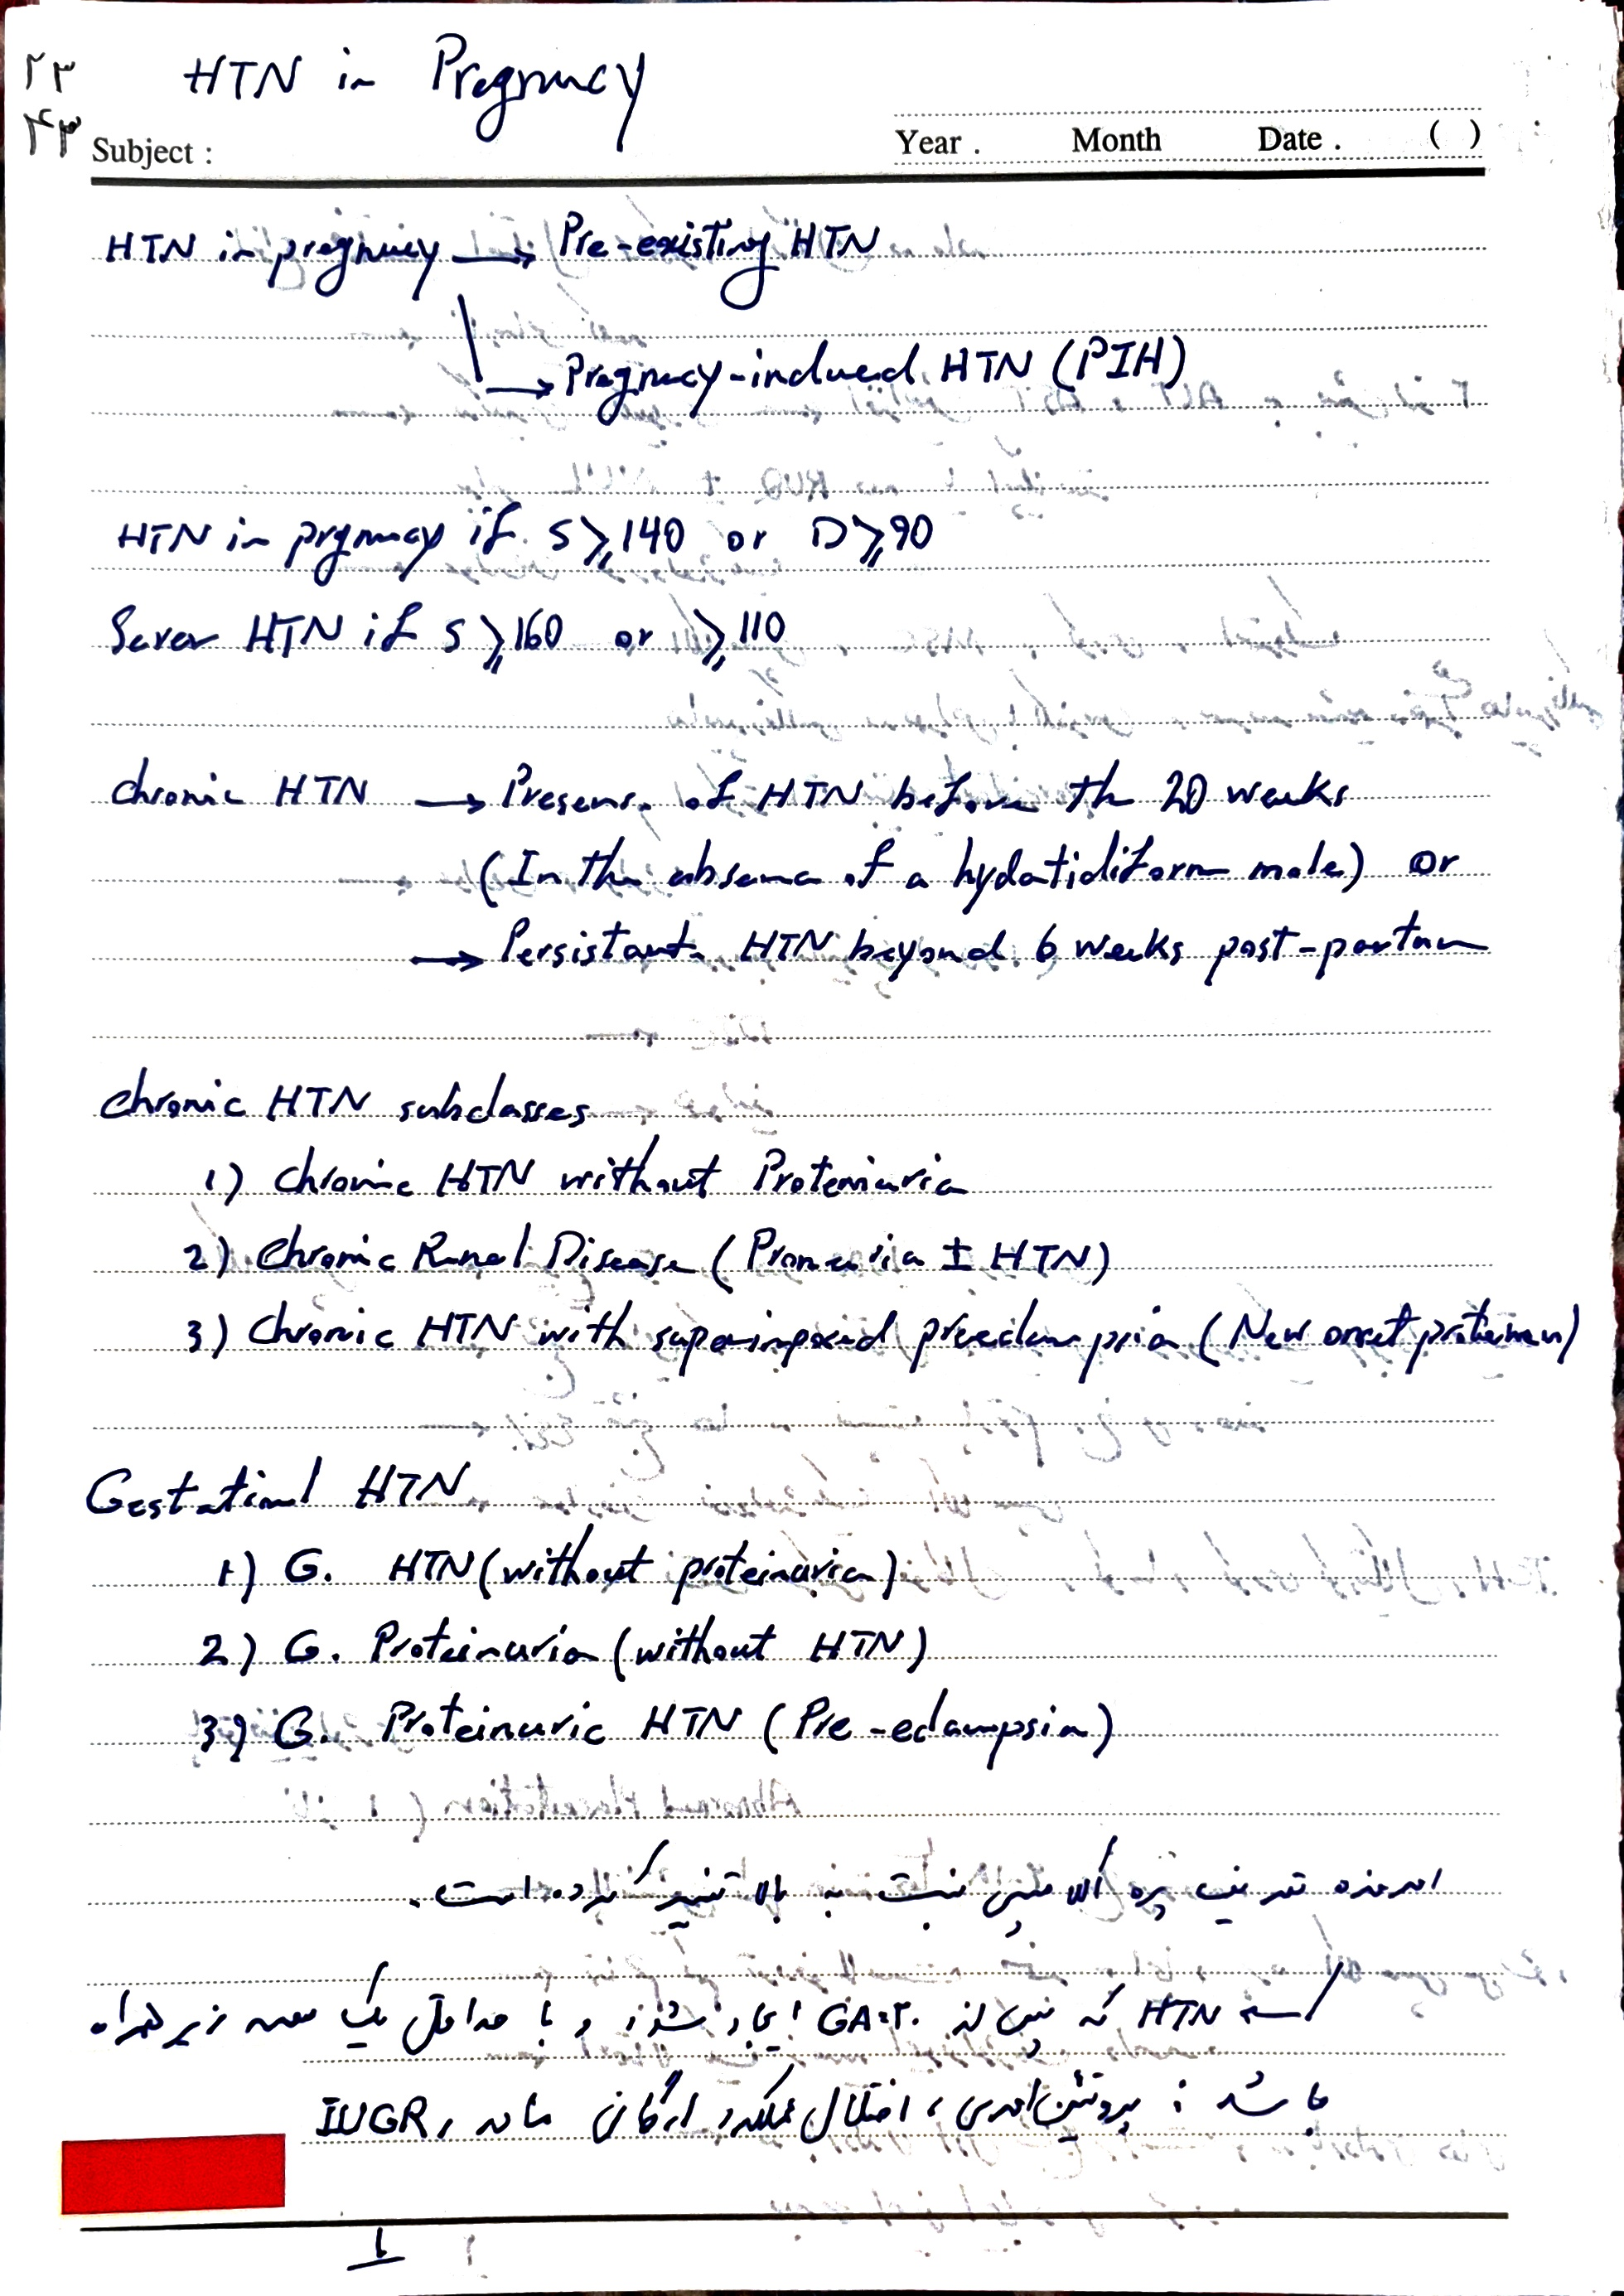
\includegraphics[width=\textwidth,height=0.86\textheight,keepaspectratio]{images/pic01.jpg}
\end{center}
% pic02.jpg = 20261013_024640458.jpg; Drive ID: 1lyG4O70cZG8ujH_JhAsqgiEi2hcLY-Yt
\clearpage
\begin{center}
\textbf{تصویر 2}\par
\lr{\detokenize{20261013_024640458.jpg}}\par
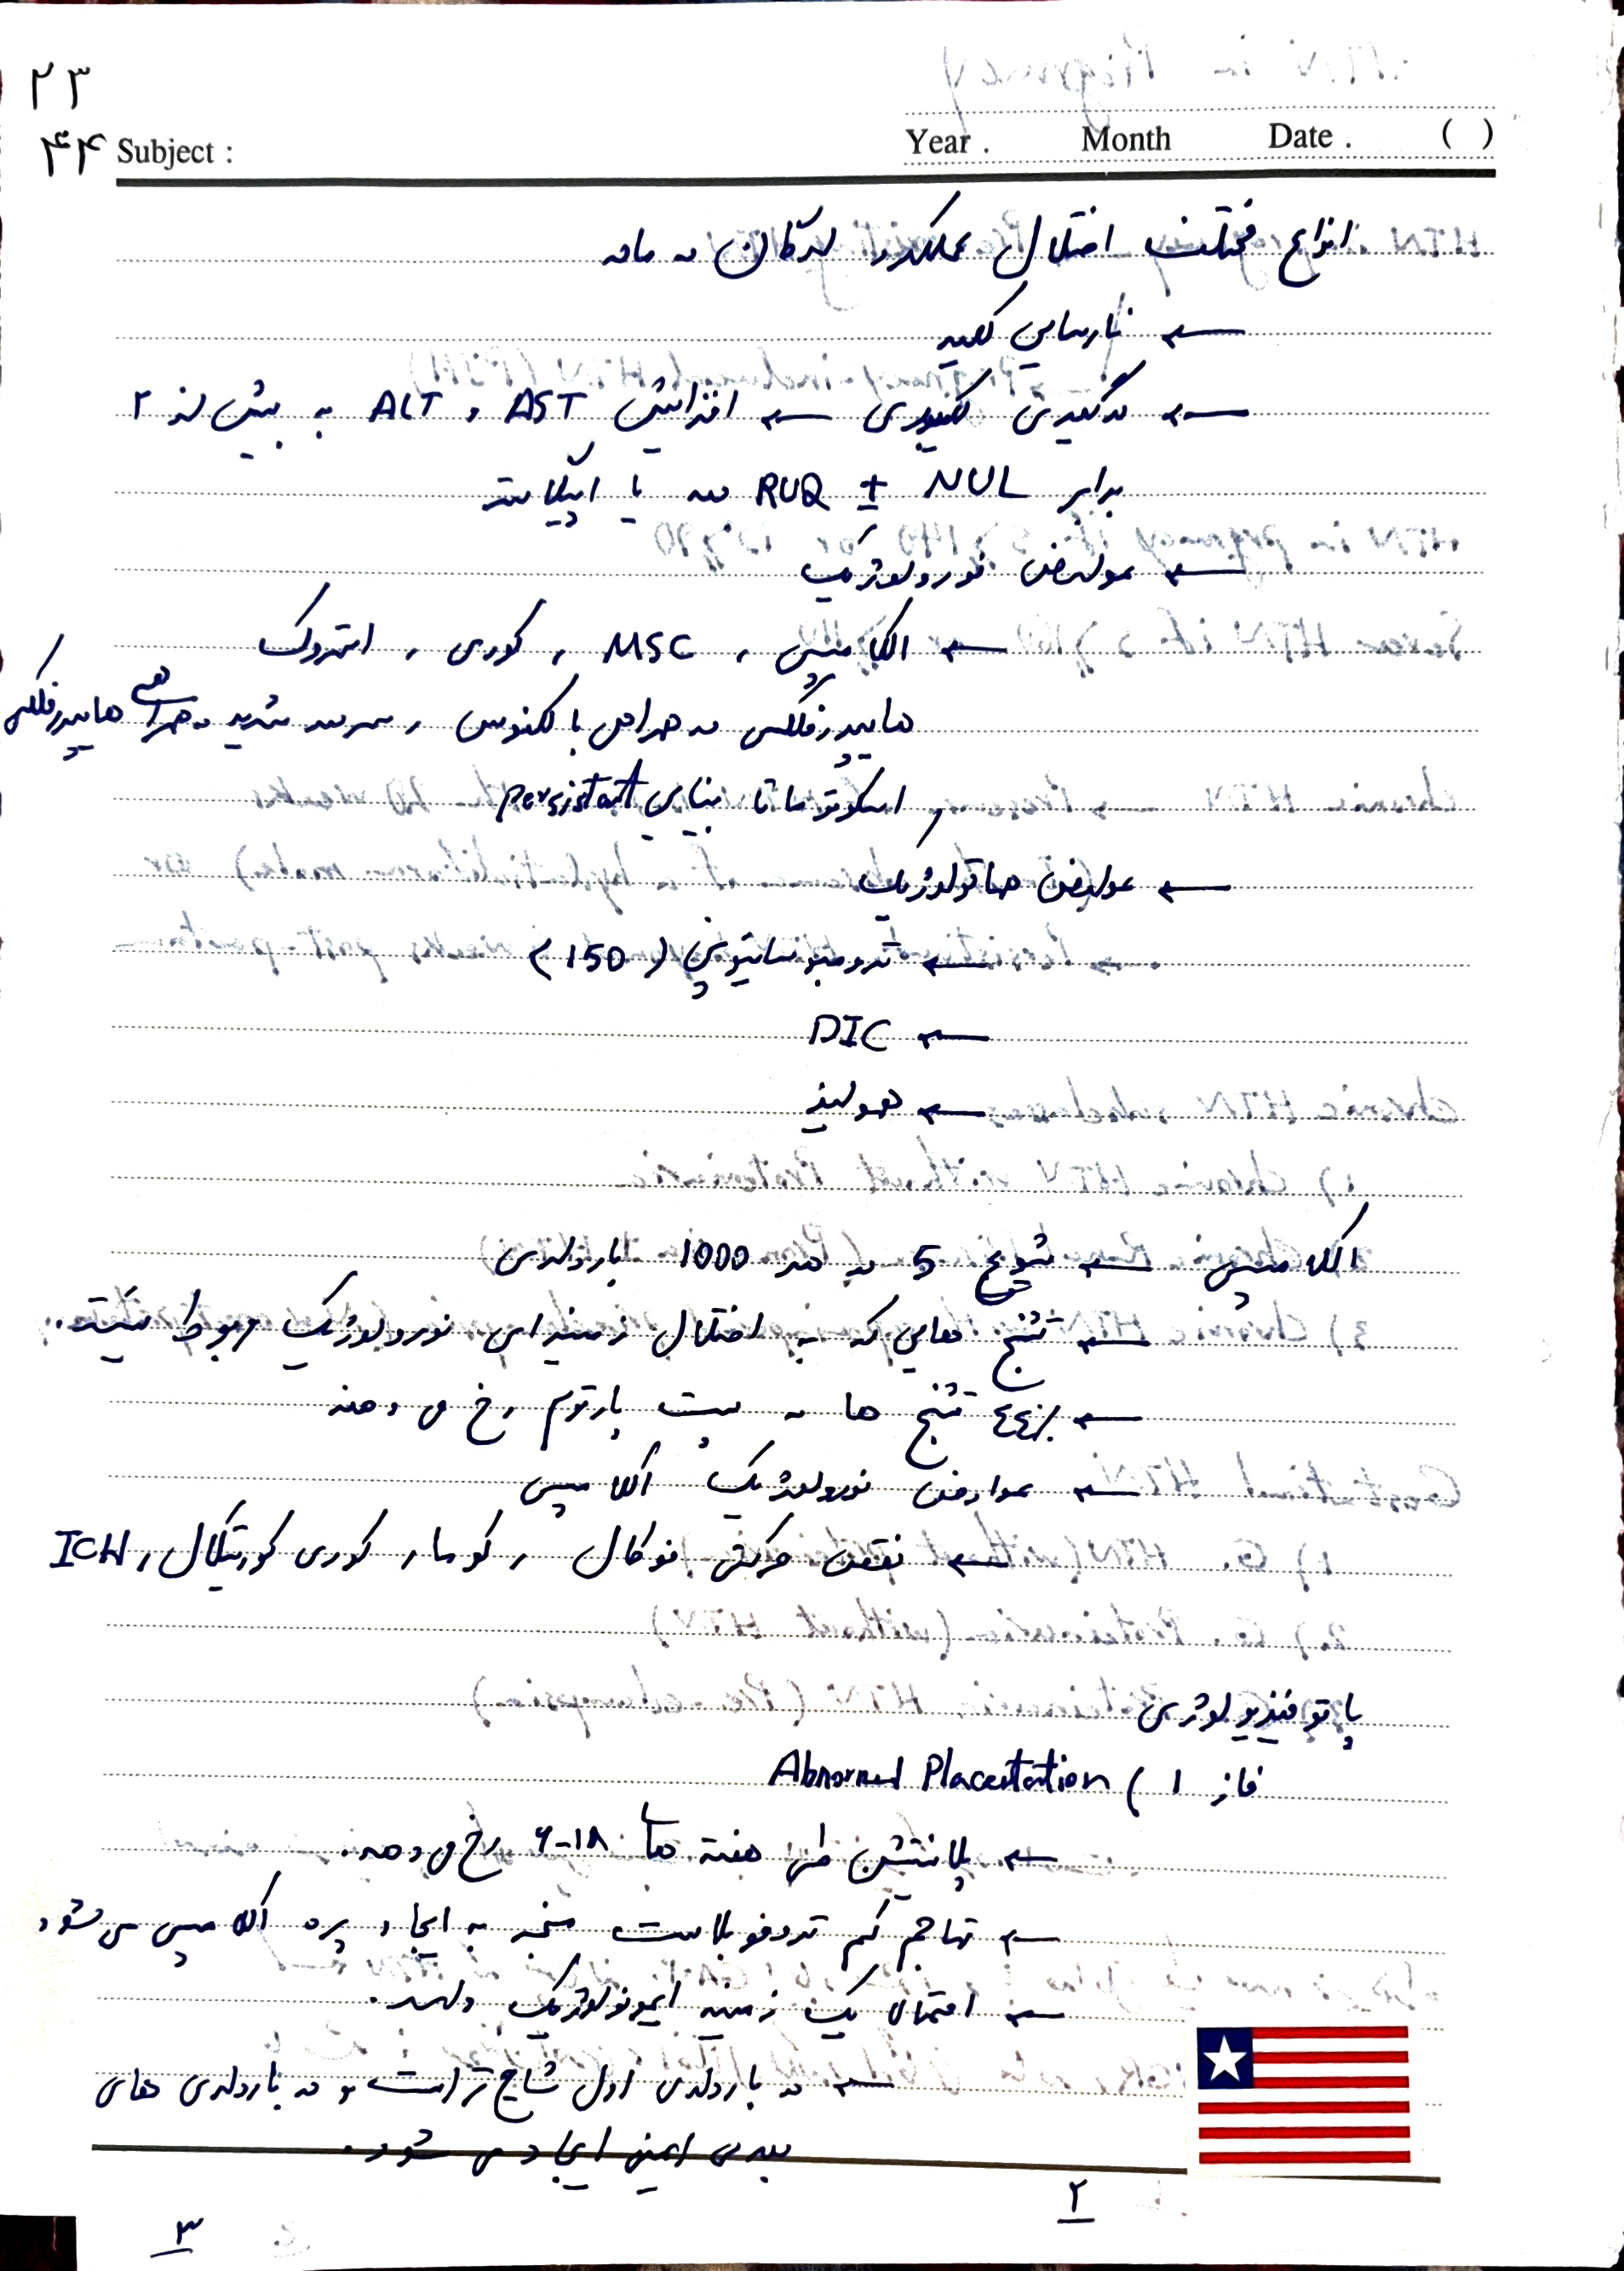
\includegraphics[width=\textwidth,height=0.86\textheight,keepaspectratio]{images/pic02.jpg}
\end{center}
% pic03.jpg = 20261013_024645417.jpg; Drive ID: 1fgrfX_hRJXszC9trKY0_wzRdrCkn54po
\clearpage
\begin{center}
\textbf{تصویر 3}\par
\lr{\detokenize{20261013_024645417.jpg}}\par
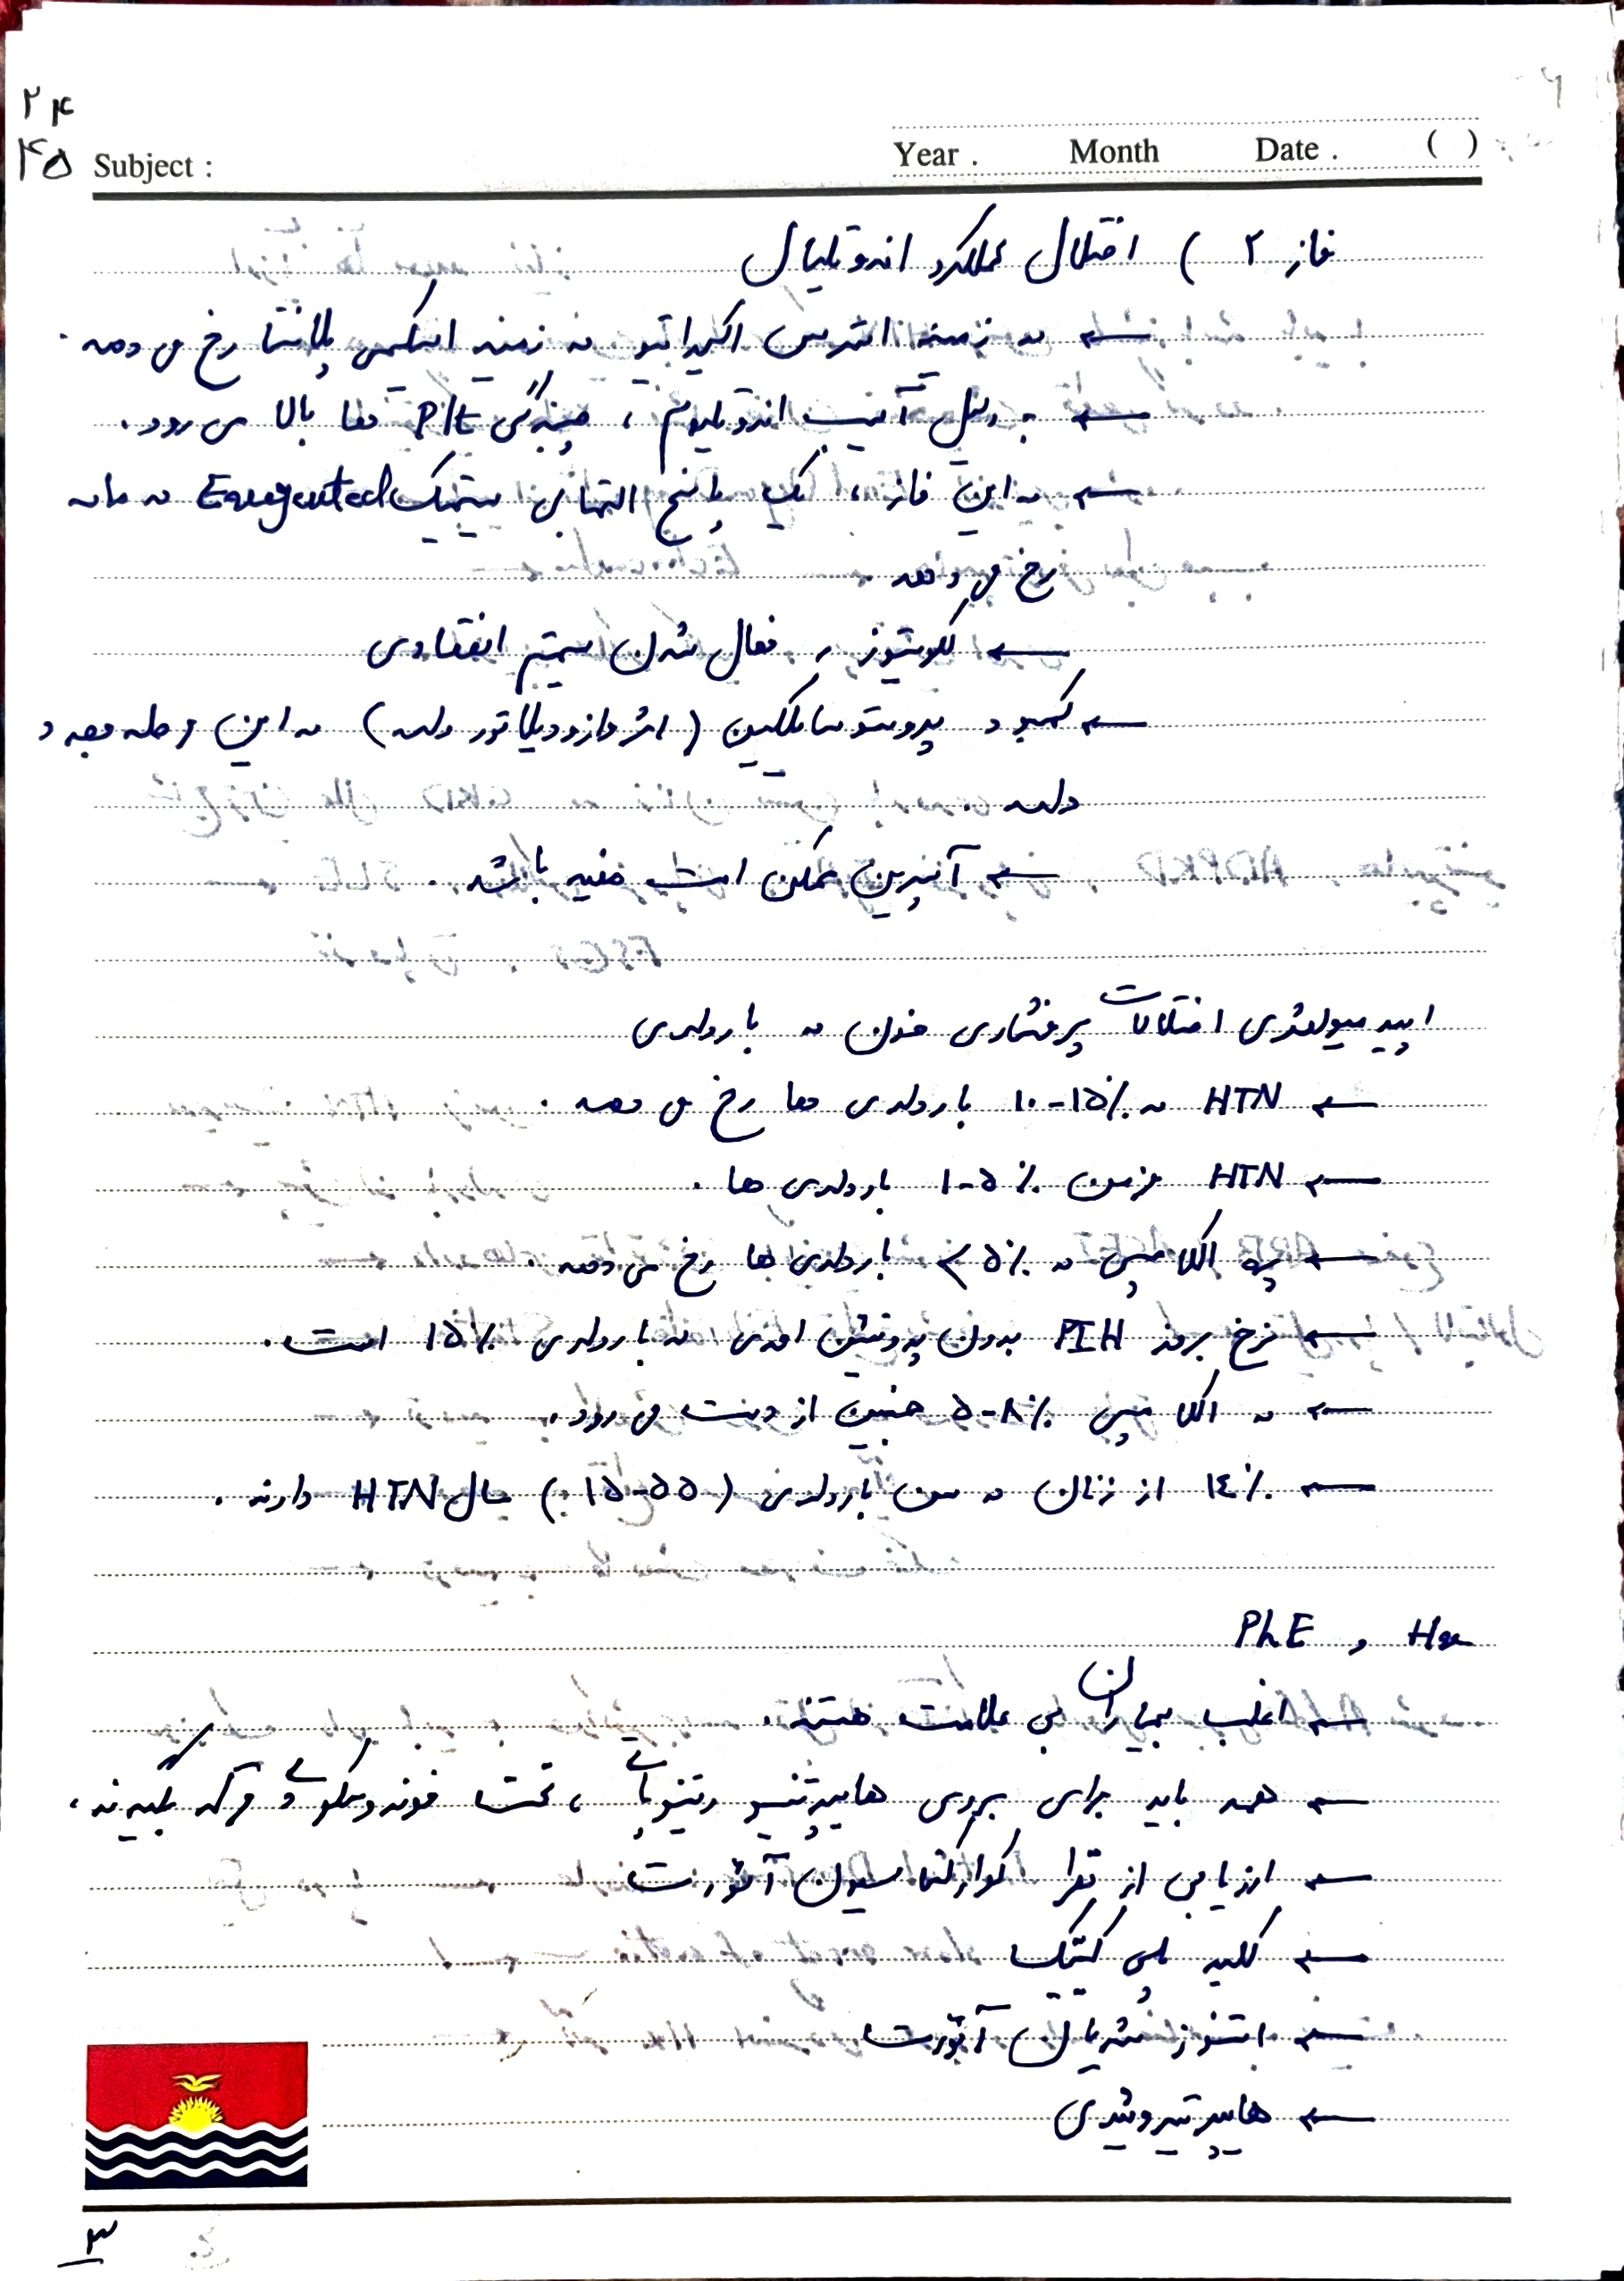
\includegraphics[width=\textwidth,height=0.86\textheight,keepaspectratio]{images/pic03.jpg}
\end{center}
% pic04.jpg = 20261013_024651115.jpg; Drive ID: 1MWs13RO3XuP5NFz4GChBXU4IVq1dTxr8
\clearpage
\begin{center}
\textbf{تصویر 4}\par
\lr{\detokenize{20261013_024651115.jpg}}\par
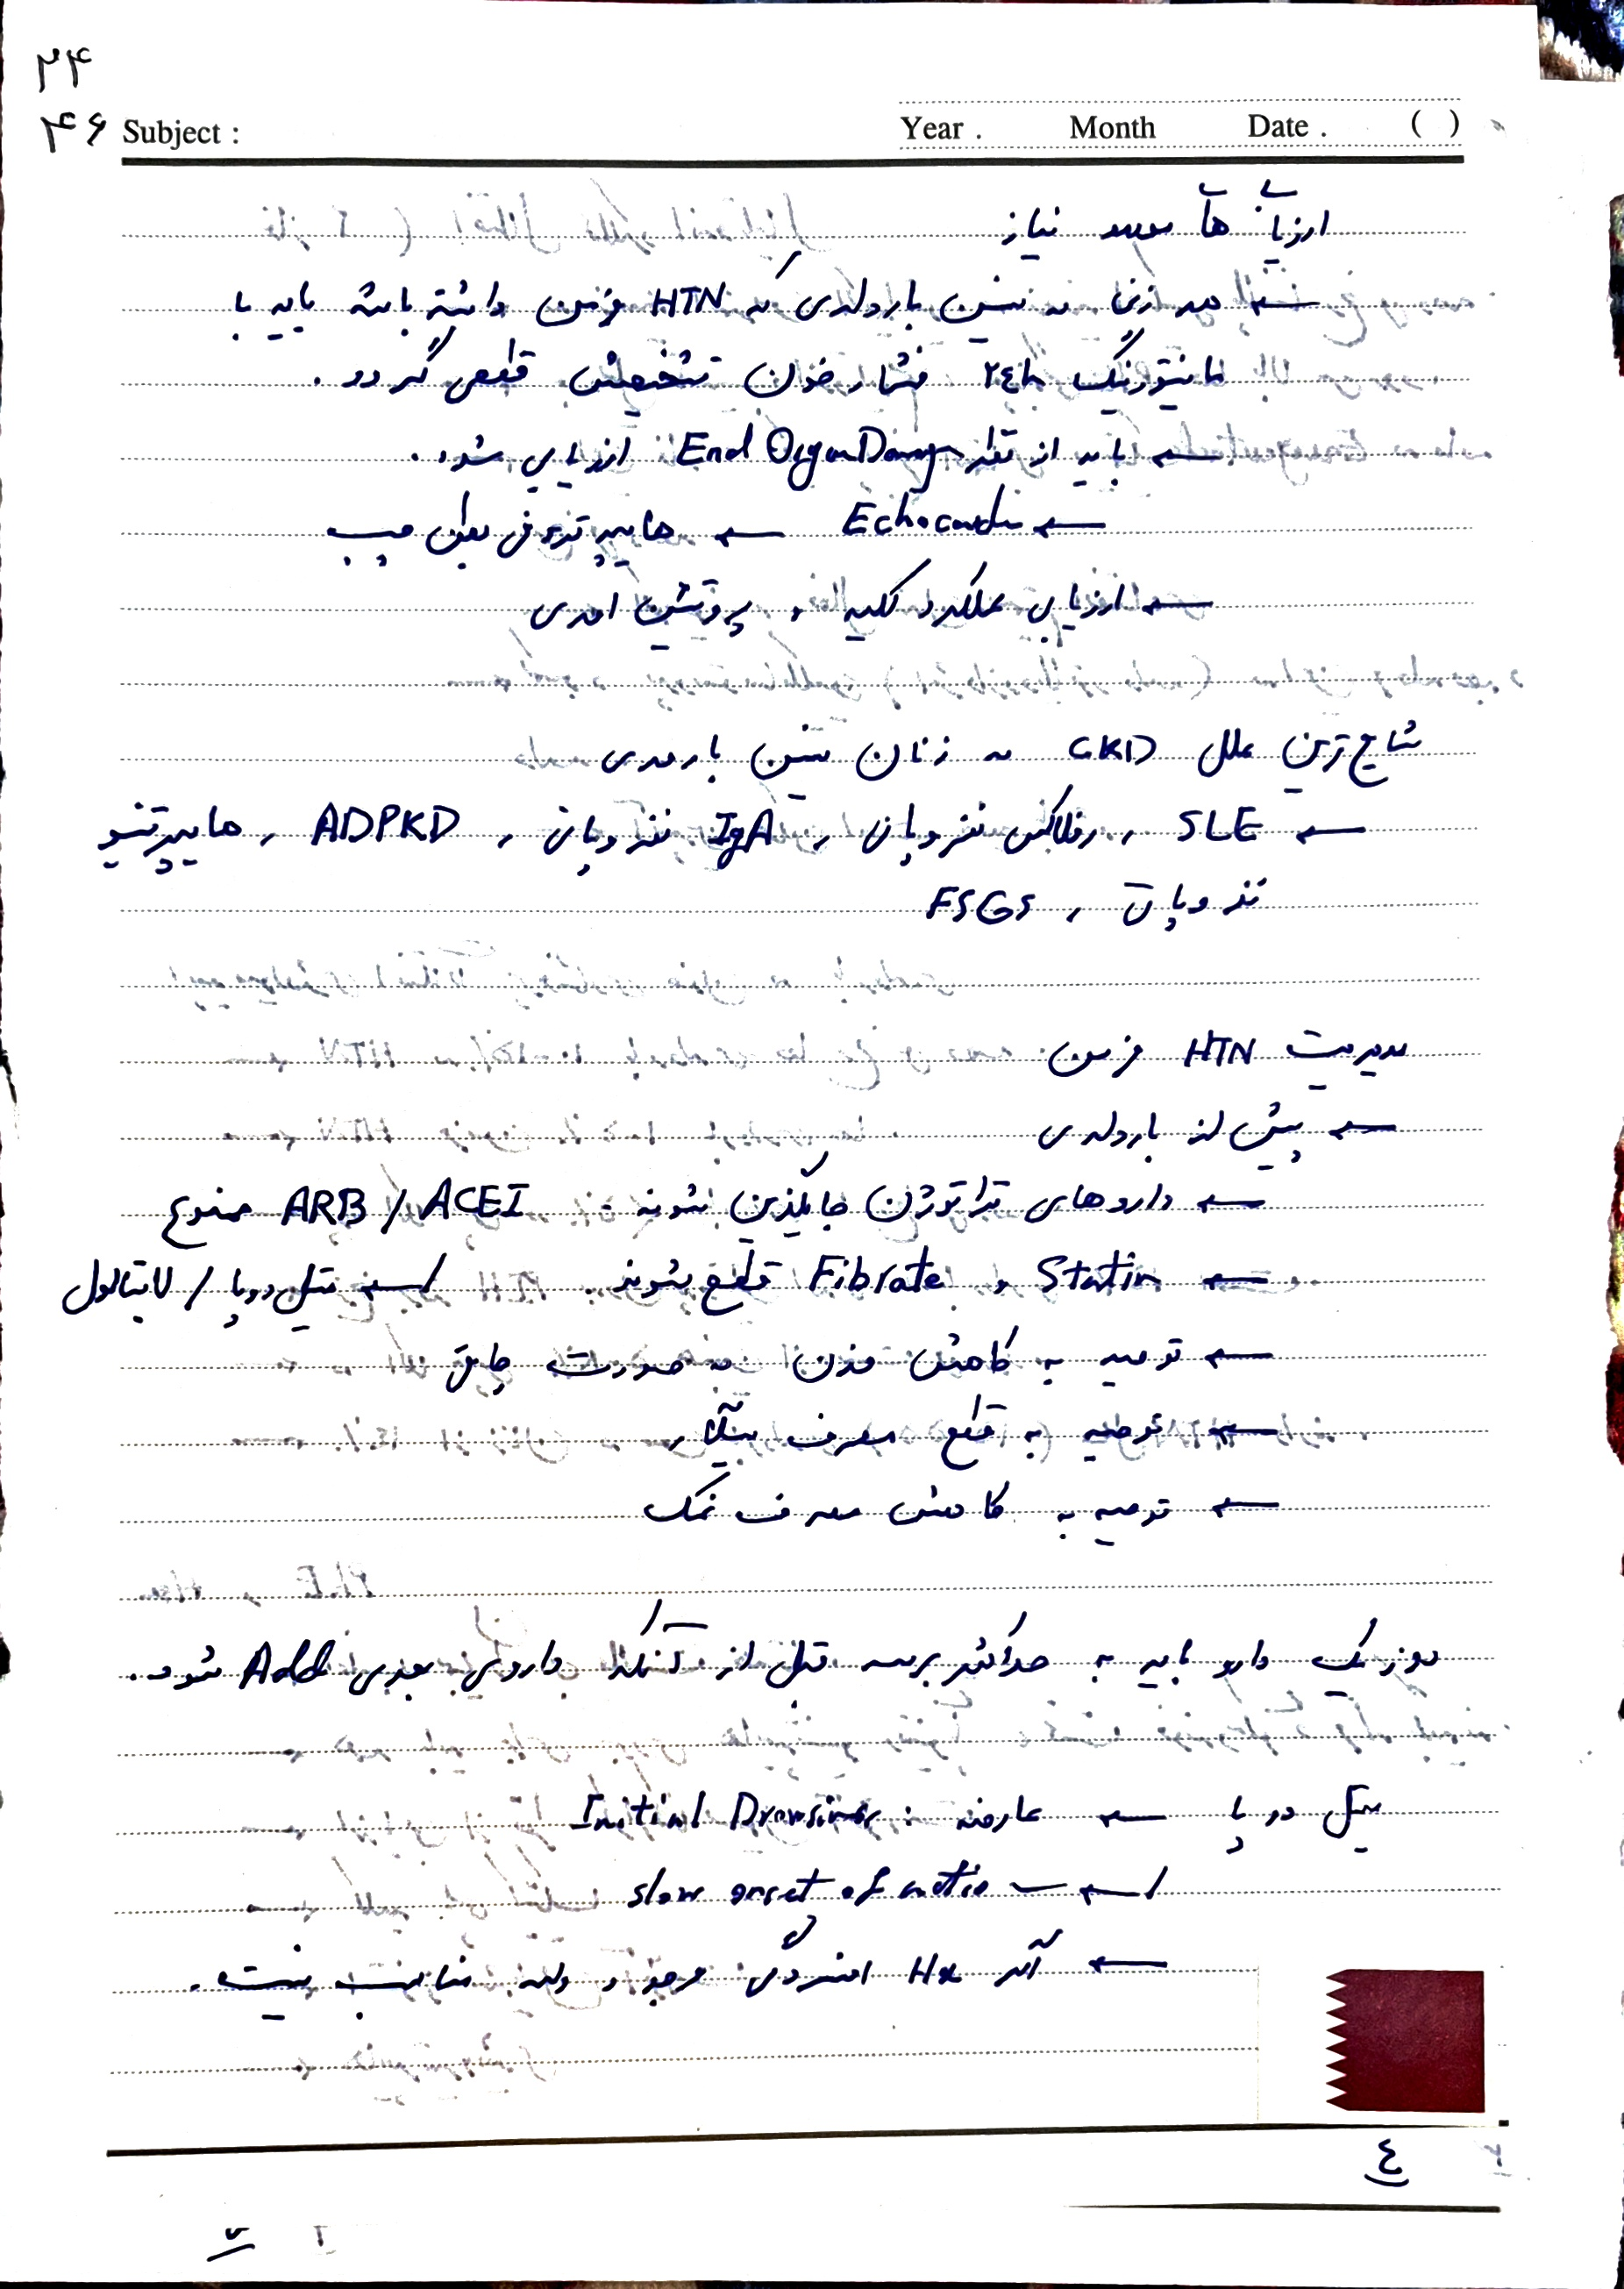
\includegraphics[width=\textwidth,height=0.86\textheight,keepaspectratio]{images/pic04.jpg}
\end{center}
% pic05.jpg = 20261013_024657910.jpg; Drive ID: 15J4kETMKV3BMelieFJipocEv1pIytltT
\clearpage
\begin{center}
\textbf{تصویر 5}\par
\lr{\detokenize{20261013_024657910.jpg}}\par
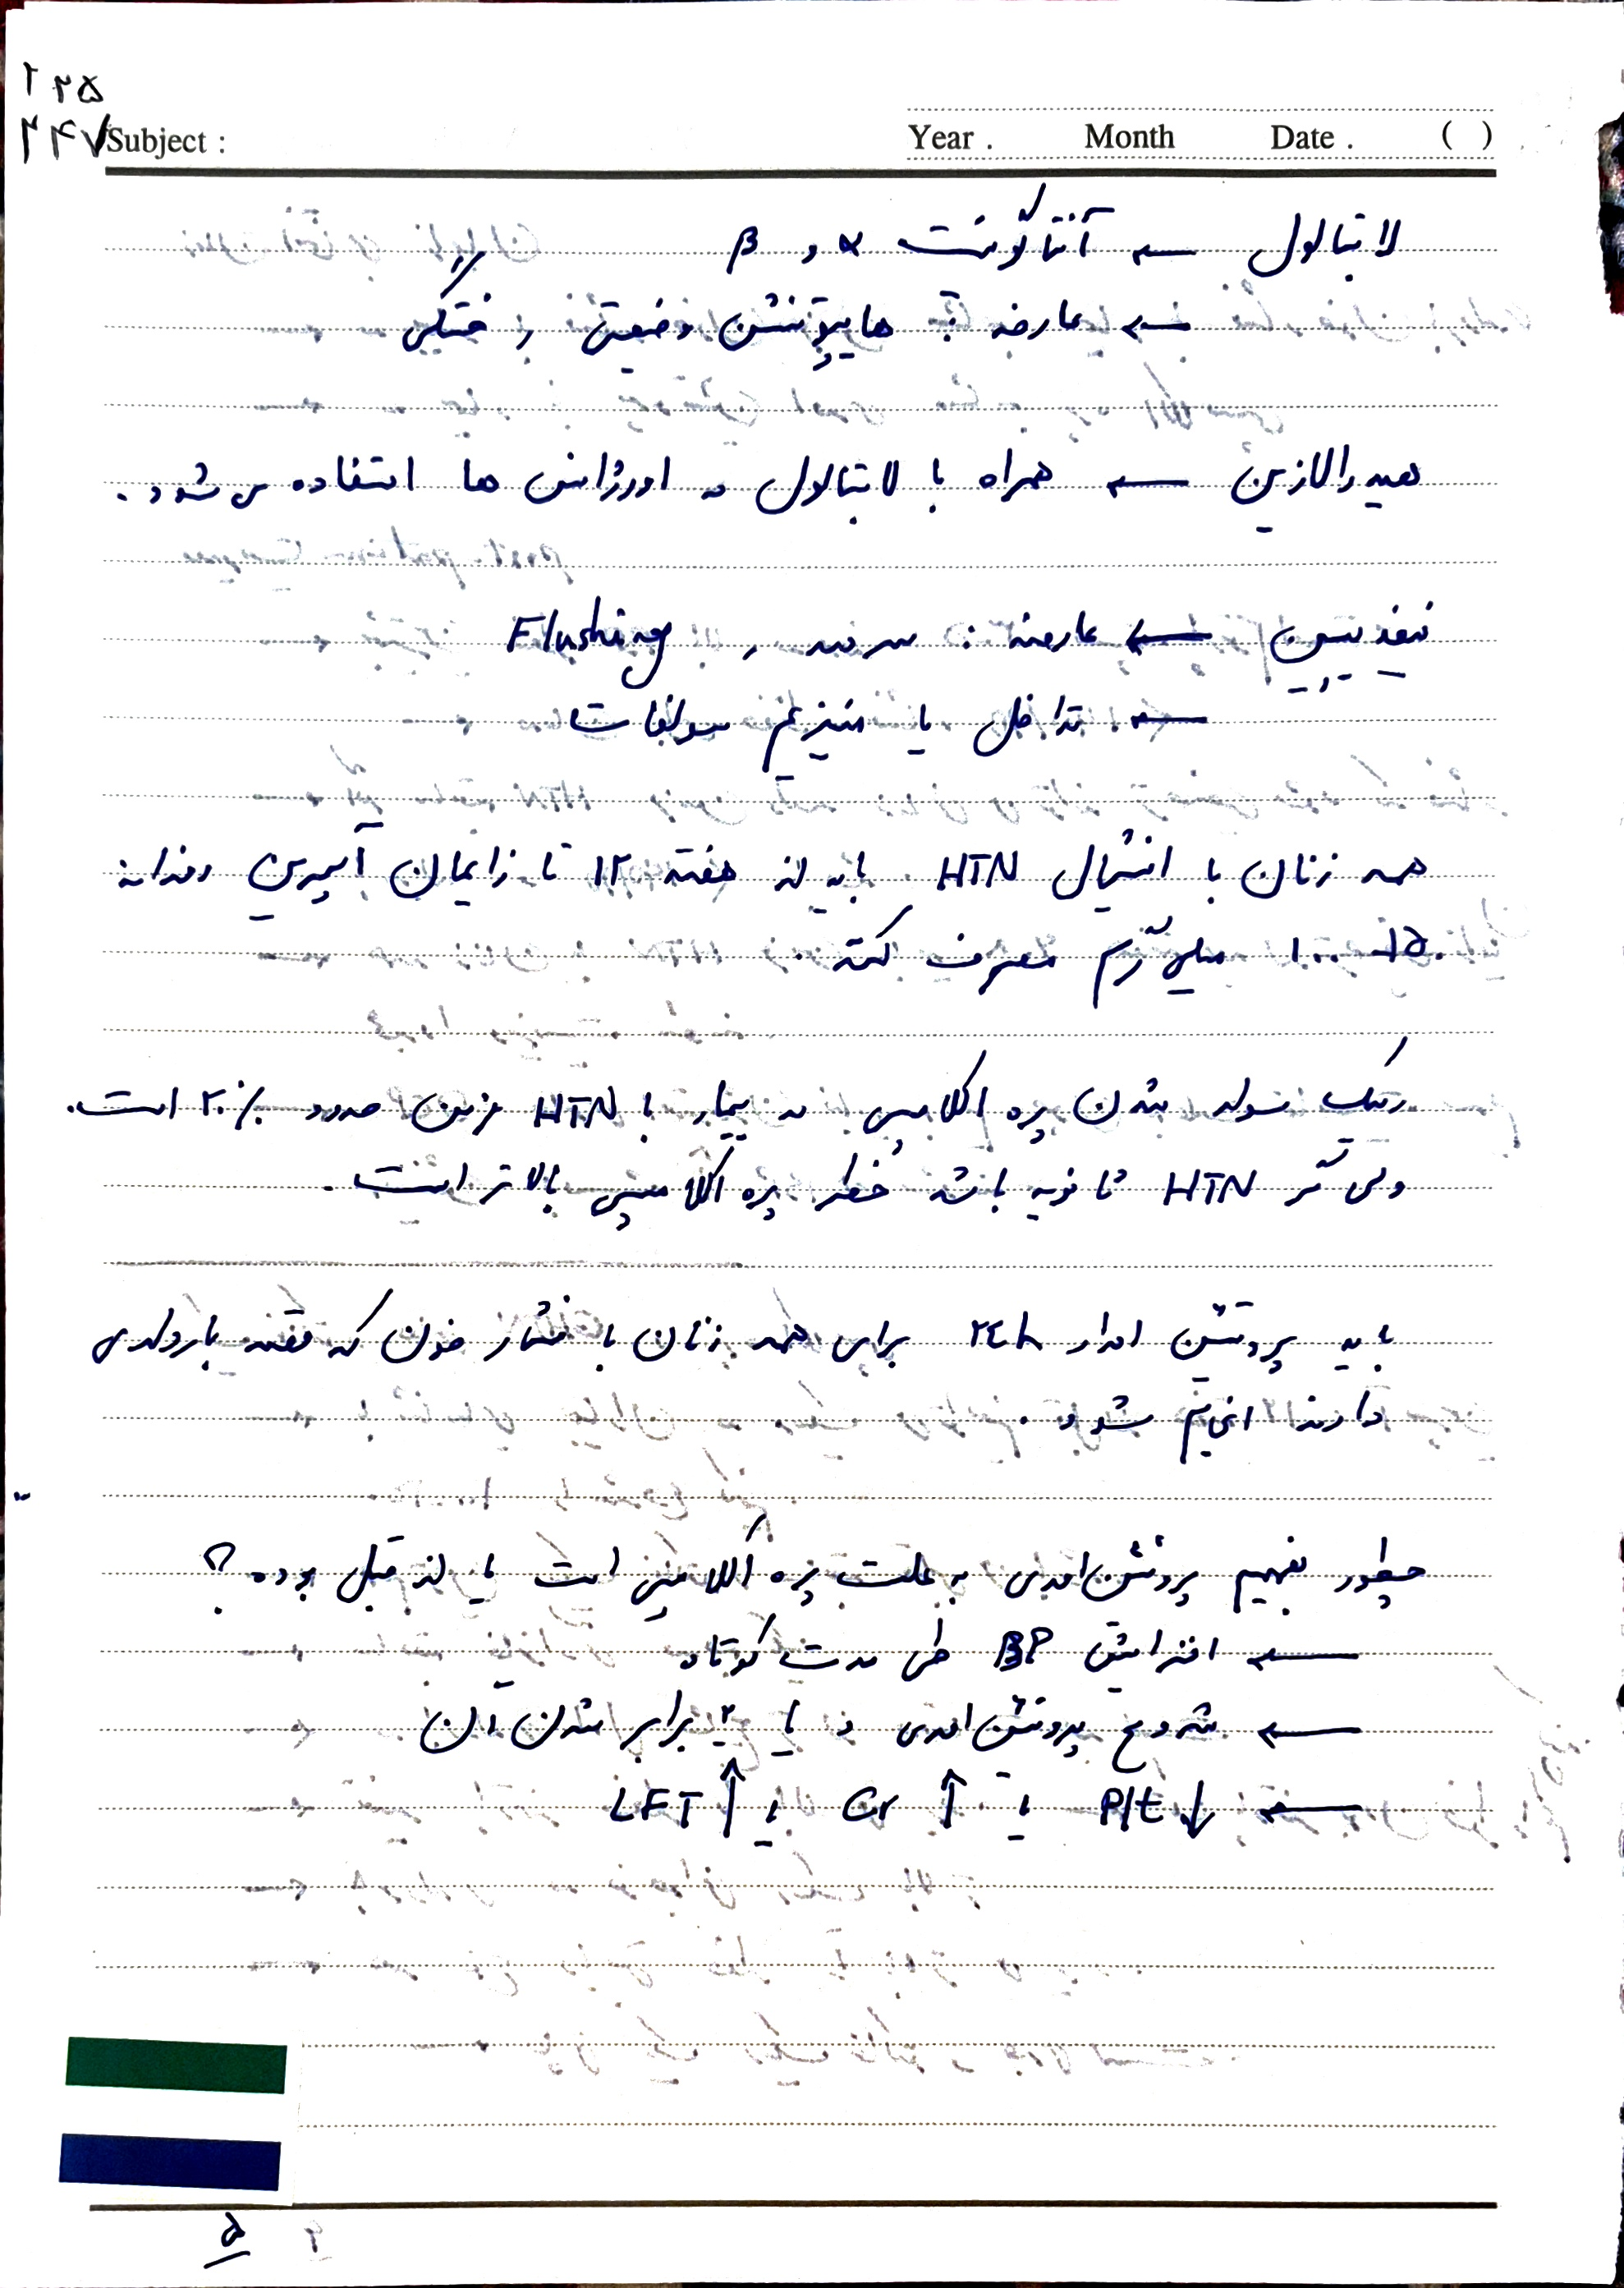
\includegraphics[width=\textwidth,height=0.86\textheight,keepaspectratio]{images/pic05.jpg}
\end{center}
% pic06.jpg = 20261013_024708278.jpg; Drive ID: 1VxJ5Q-96VdyAB5fnFJmtcCfyxijXgWTj
\clearpage
\begin{center}
\textbf{تصویر 6}\par
\lr{\detokenize{20261013_024708278.jpg}}\par
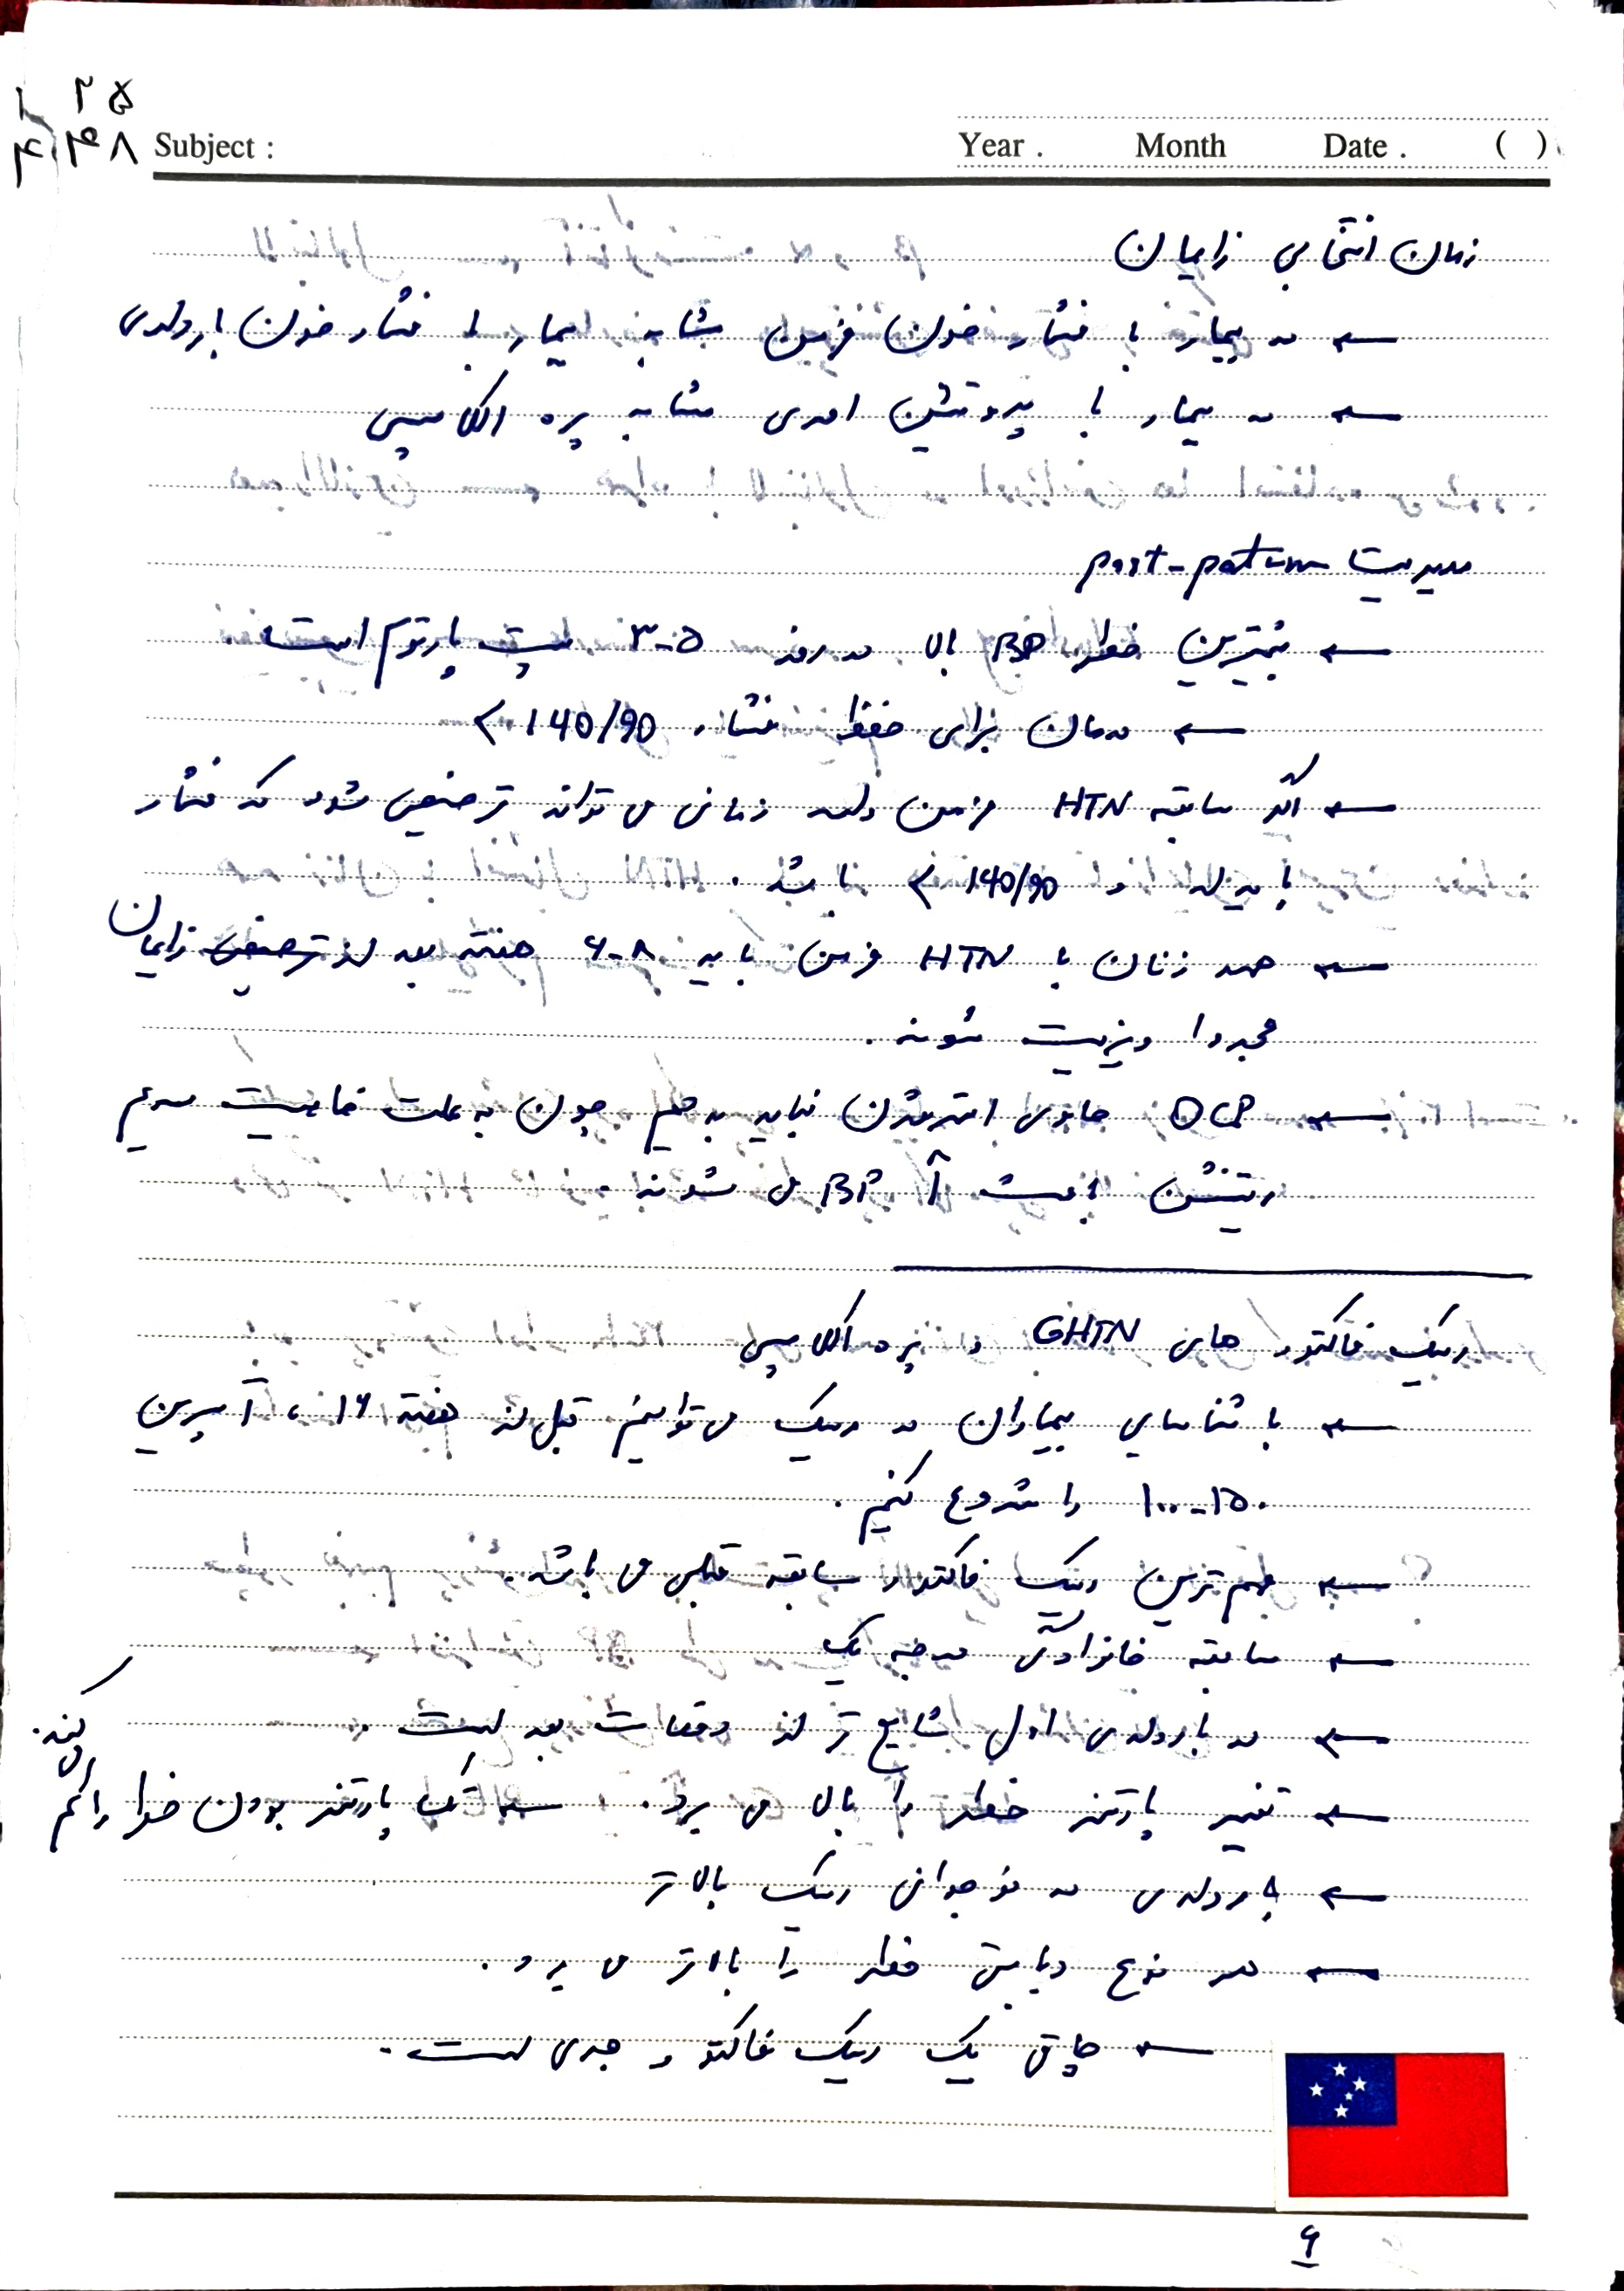
\includegraphics[width=\textwidth,height=0.86\textheight,keepaspectratio]{images/pic06.jpg}
\end{center}
% pic07.jpg = 20261013_024713314.jpg; Drive ID: 1NuaLss3lcATKQGryvQLyPo2oznTStXuj
\clearpage
\begin{center}
\textbf{تصویر 7}\par
\lr{\detokenize{20261013_024713314.jpg}}\par
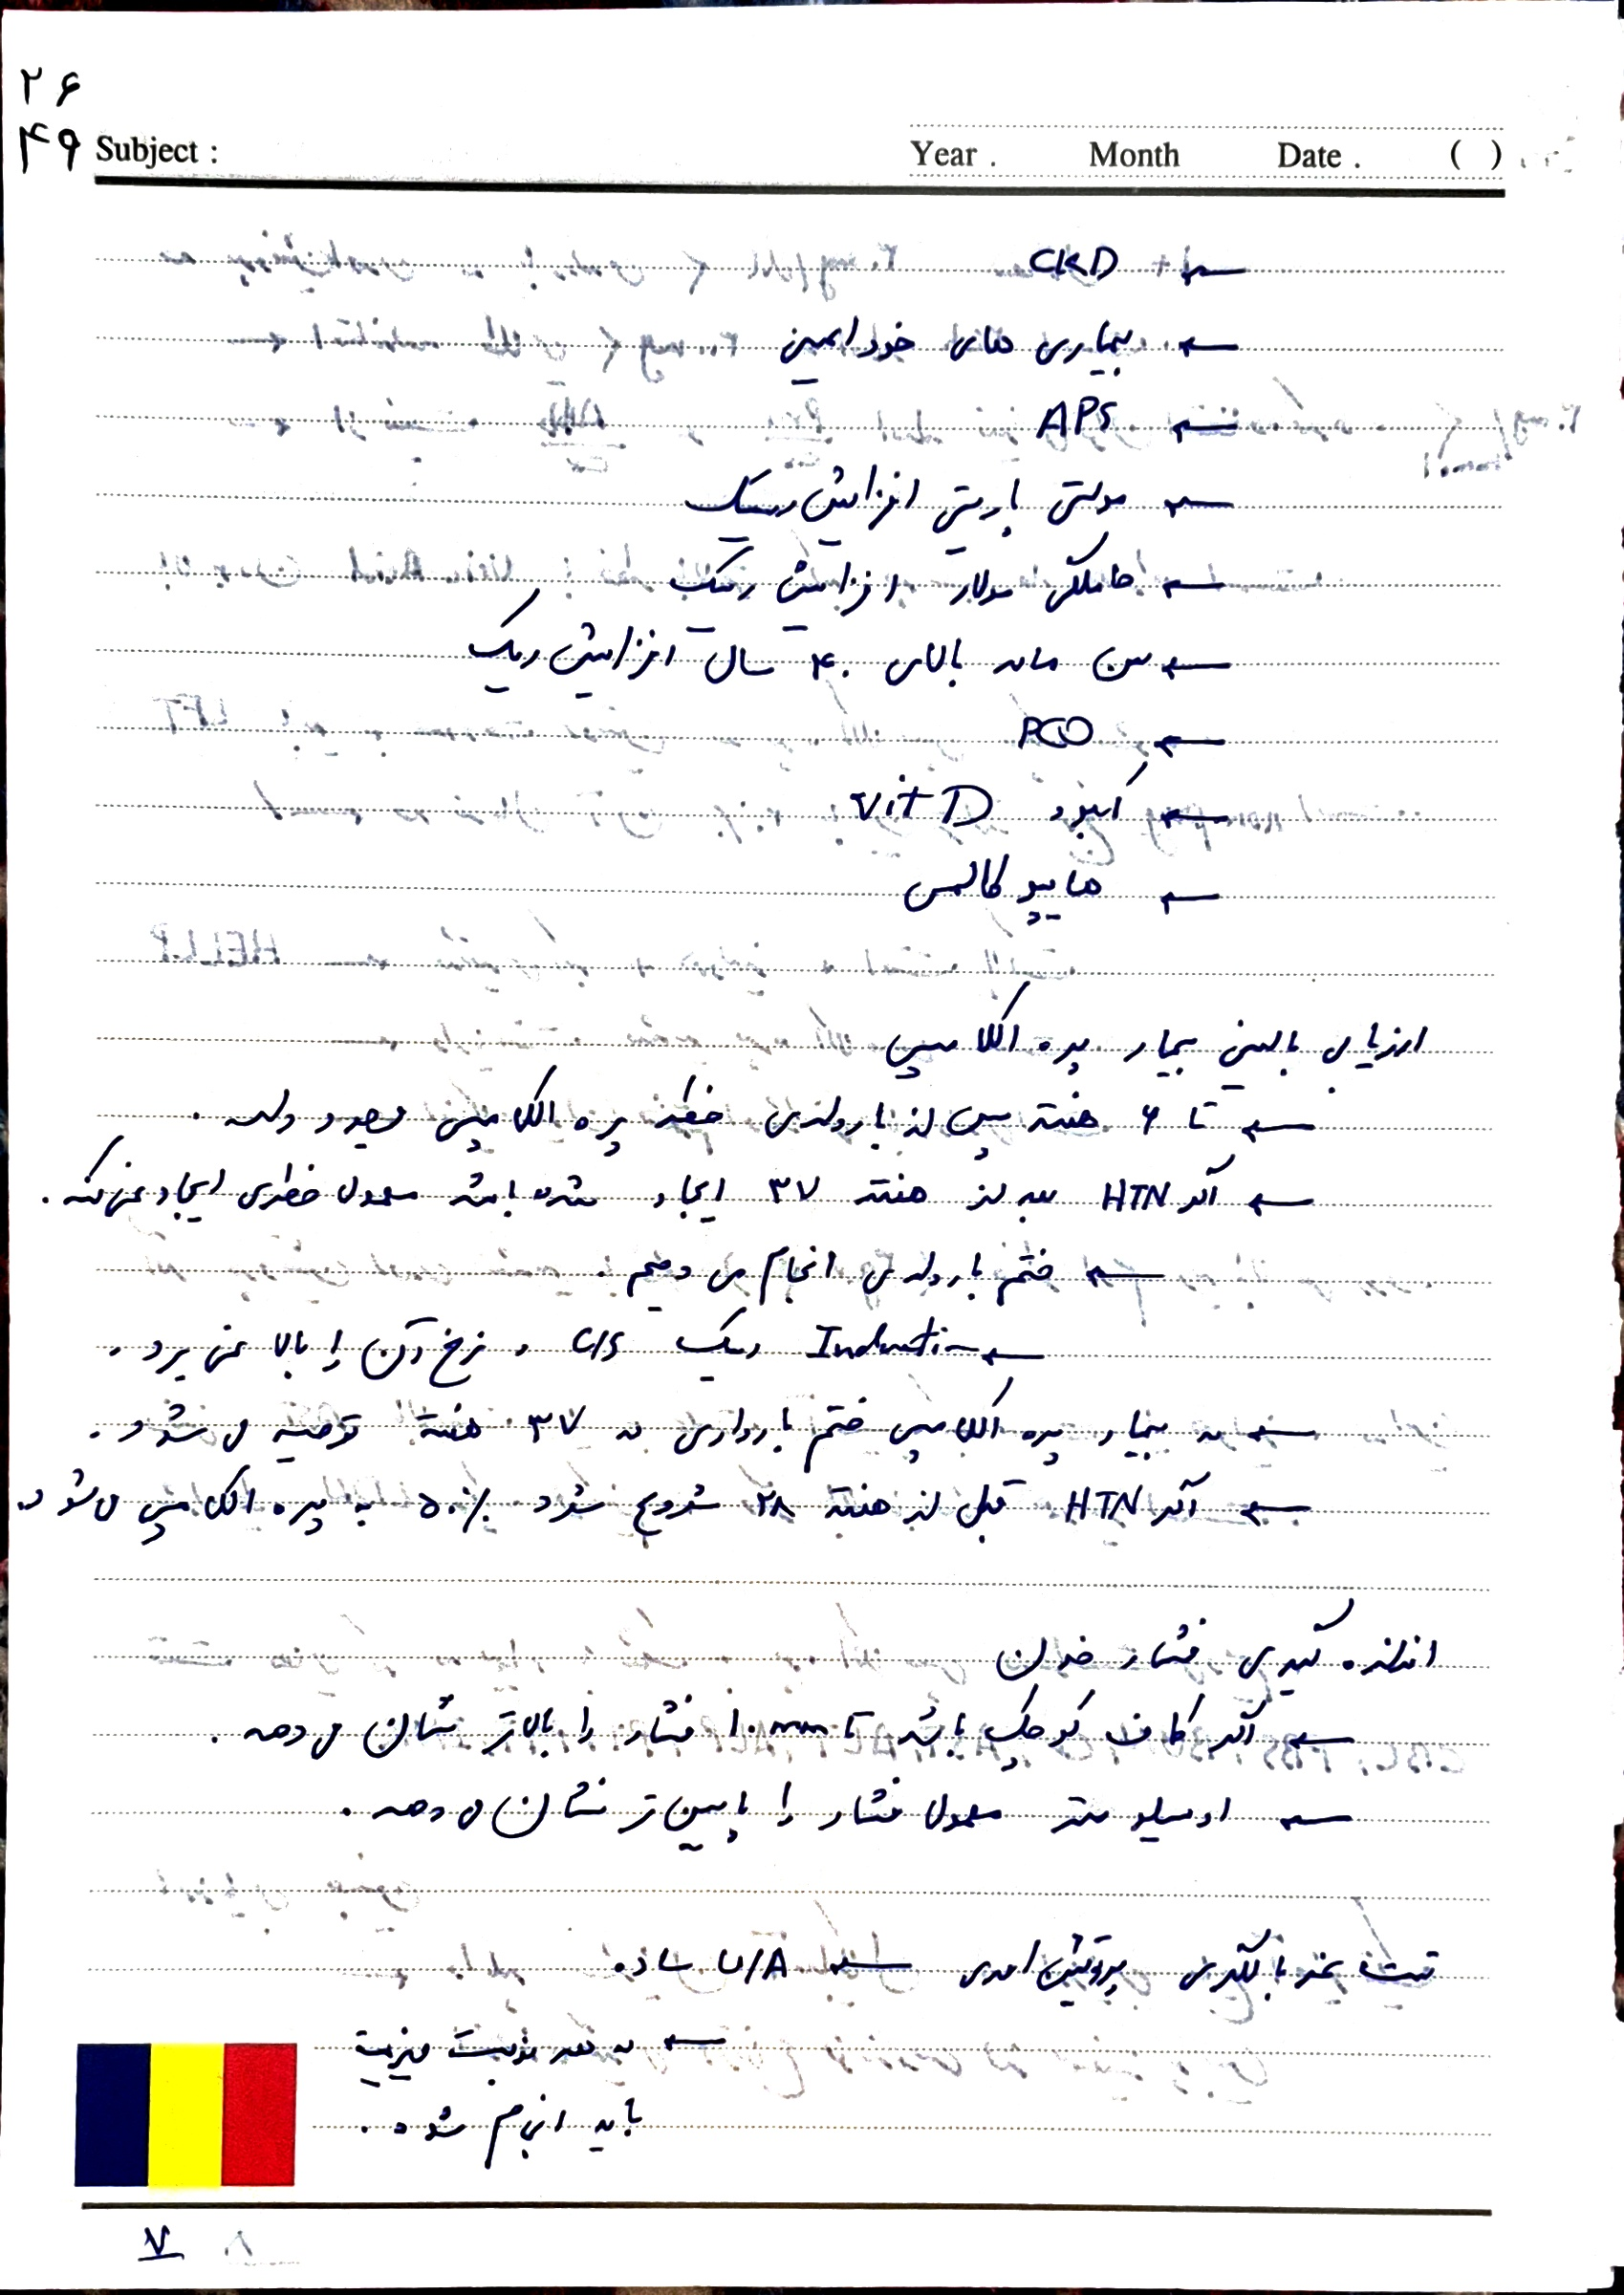
\includegraphics[width=\textwidth,height=0.86\textheight,keepaspectratio]{images/pic07.jpg}
\end{center}
% pic08.jpg = 20261013_024718627.jpg; Drive ID: 1LRly7YgcRAmN6q-KuNvblm4w5BMTGeAP
\clearpage
\begin{center}
\textbf{تصویر 8}\par
\lr{\detokenize{20261013_024718627.jpg}}\par
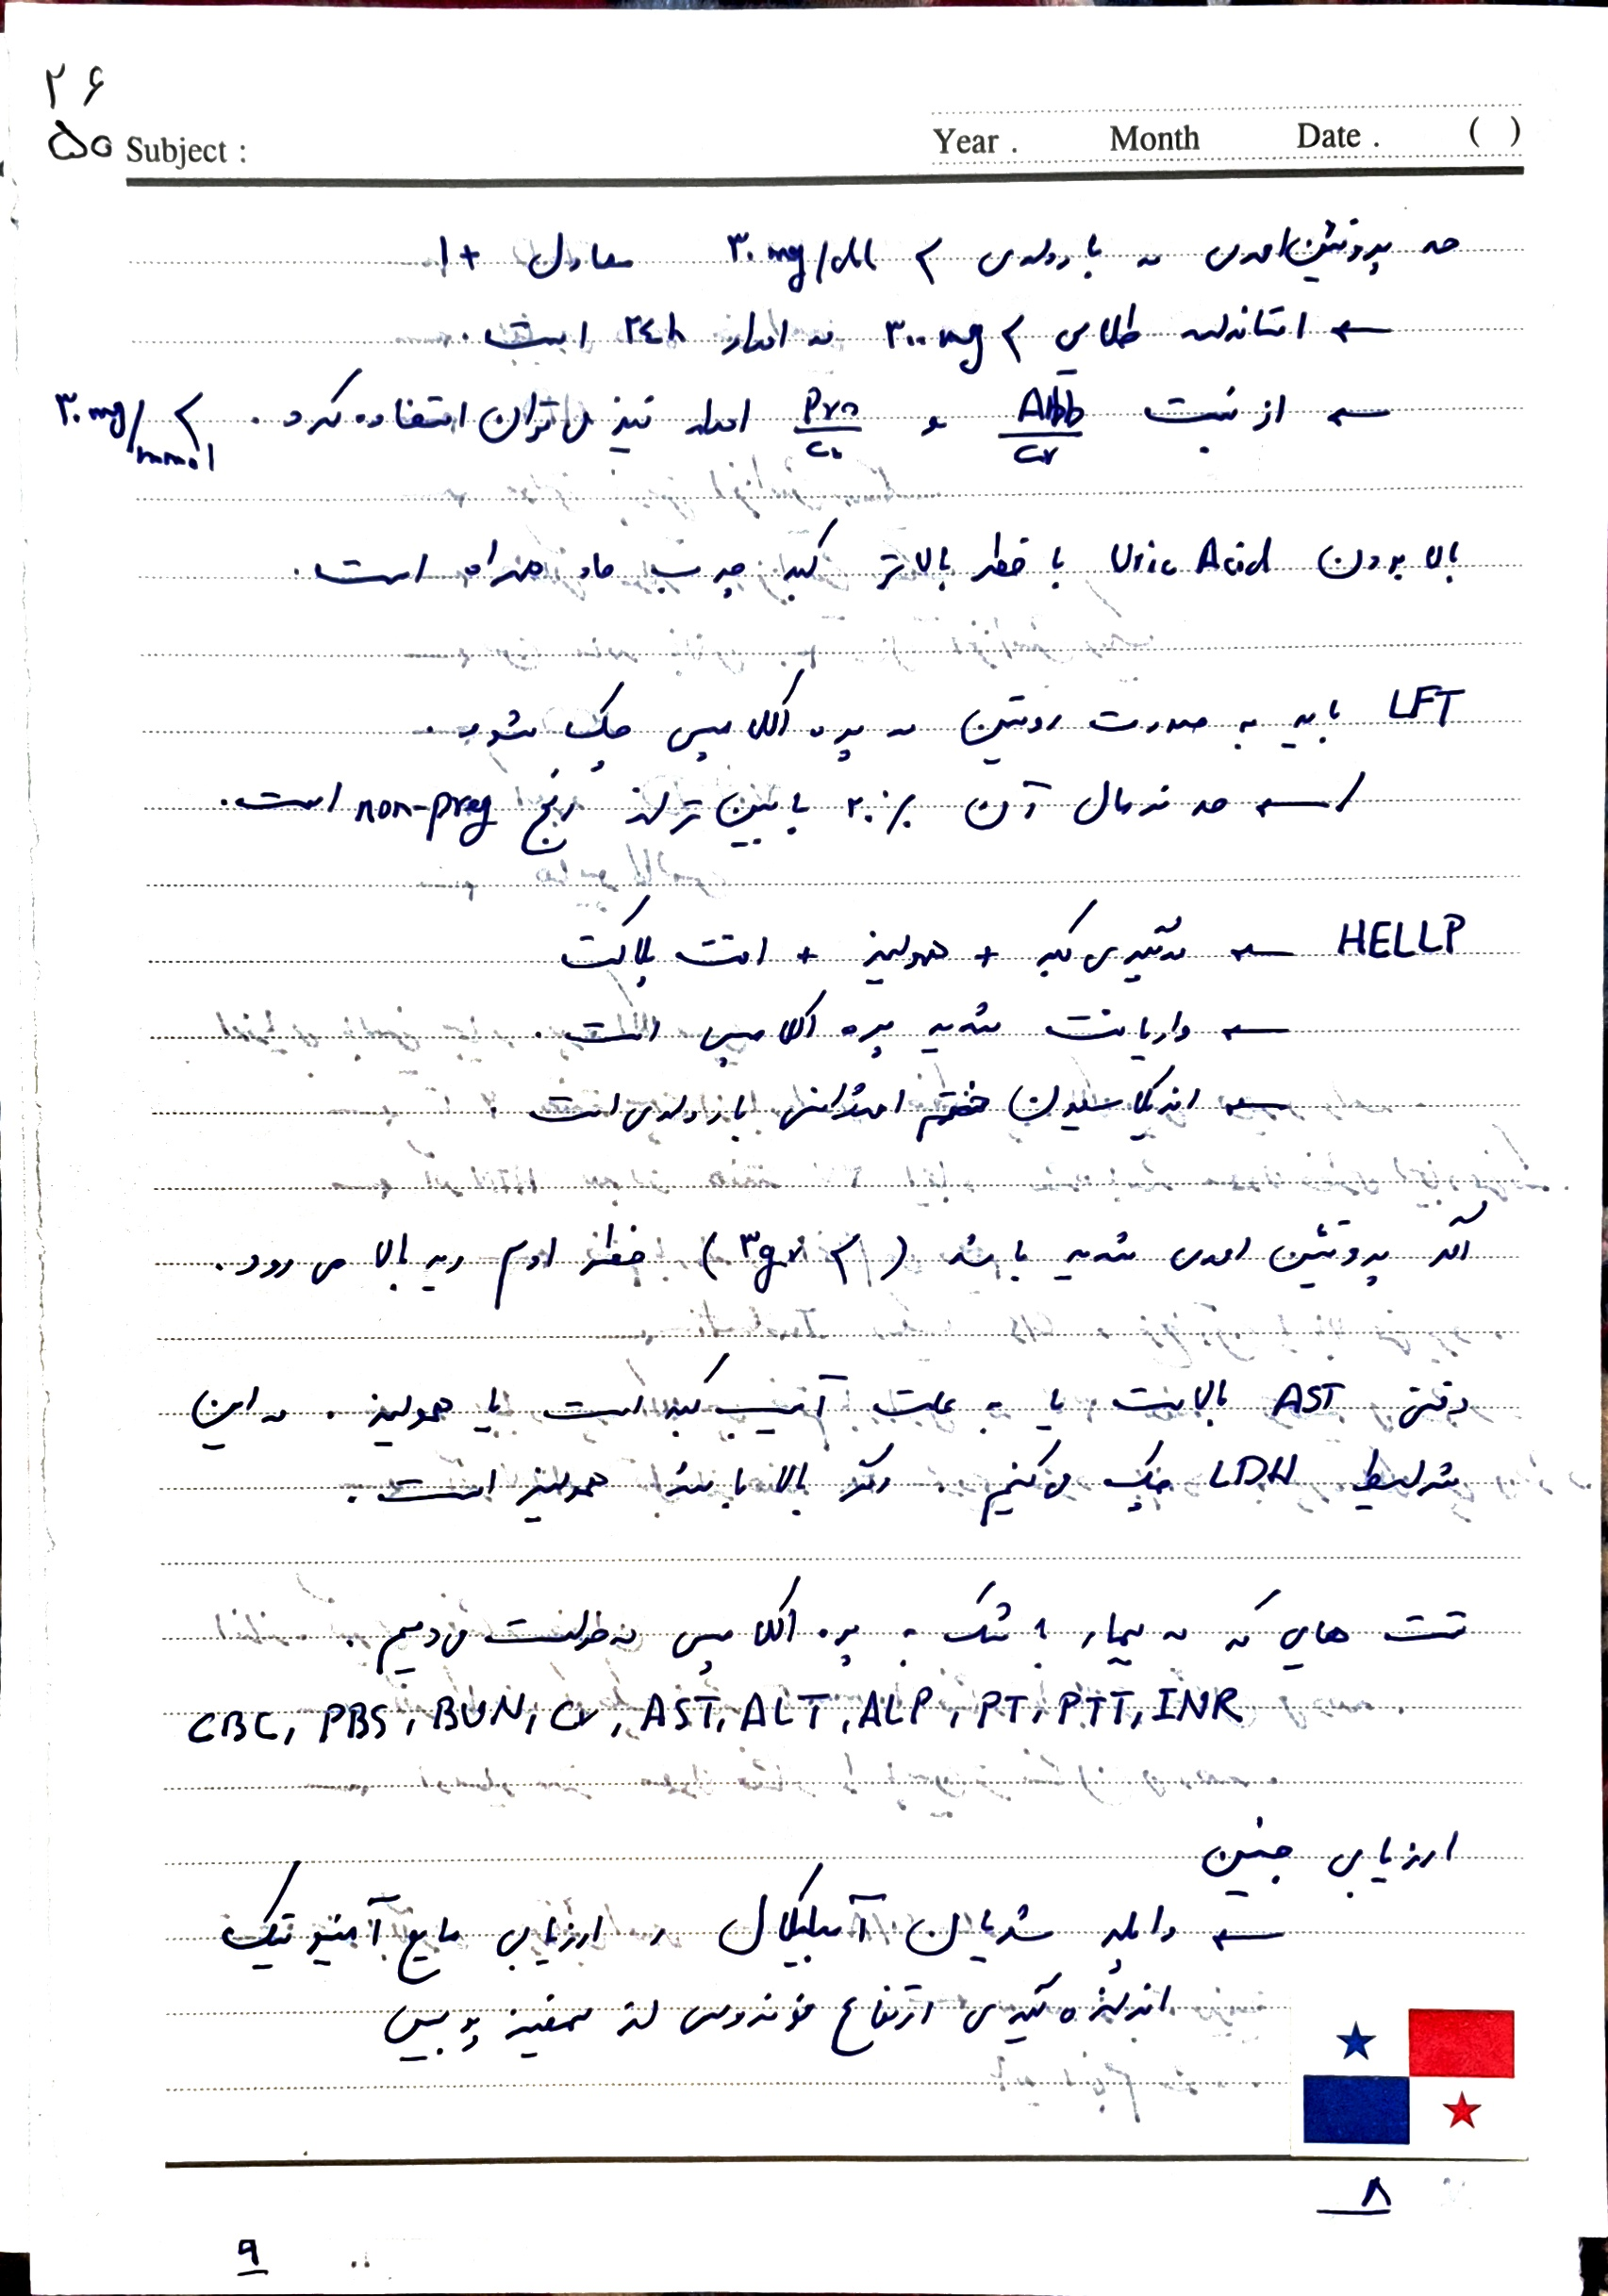
\includegraphics[width=\textwidth,height=0.86\textheight,keepaspectratio]{images/pic08.jpg}
\end{center}
% pic09.jpg = 20261013_024724432.jpg; Drive ID: 1ImzS4dIljPcSN3zA2zYXCxnh7UQ7LuUn
\clearpage
\begin{center}
\textbf{تصویر 9}\par
\lr{\detokenize{20261013_024724432.jpg}}\par
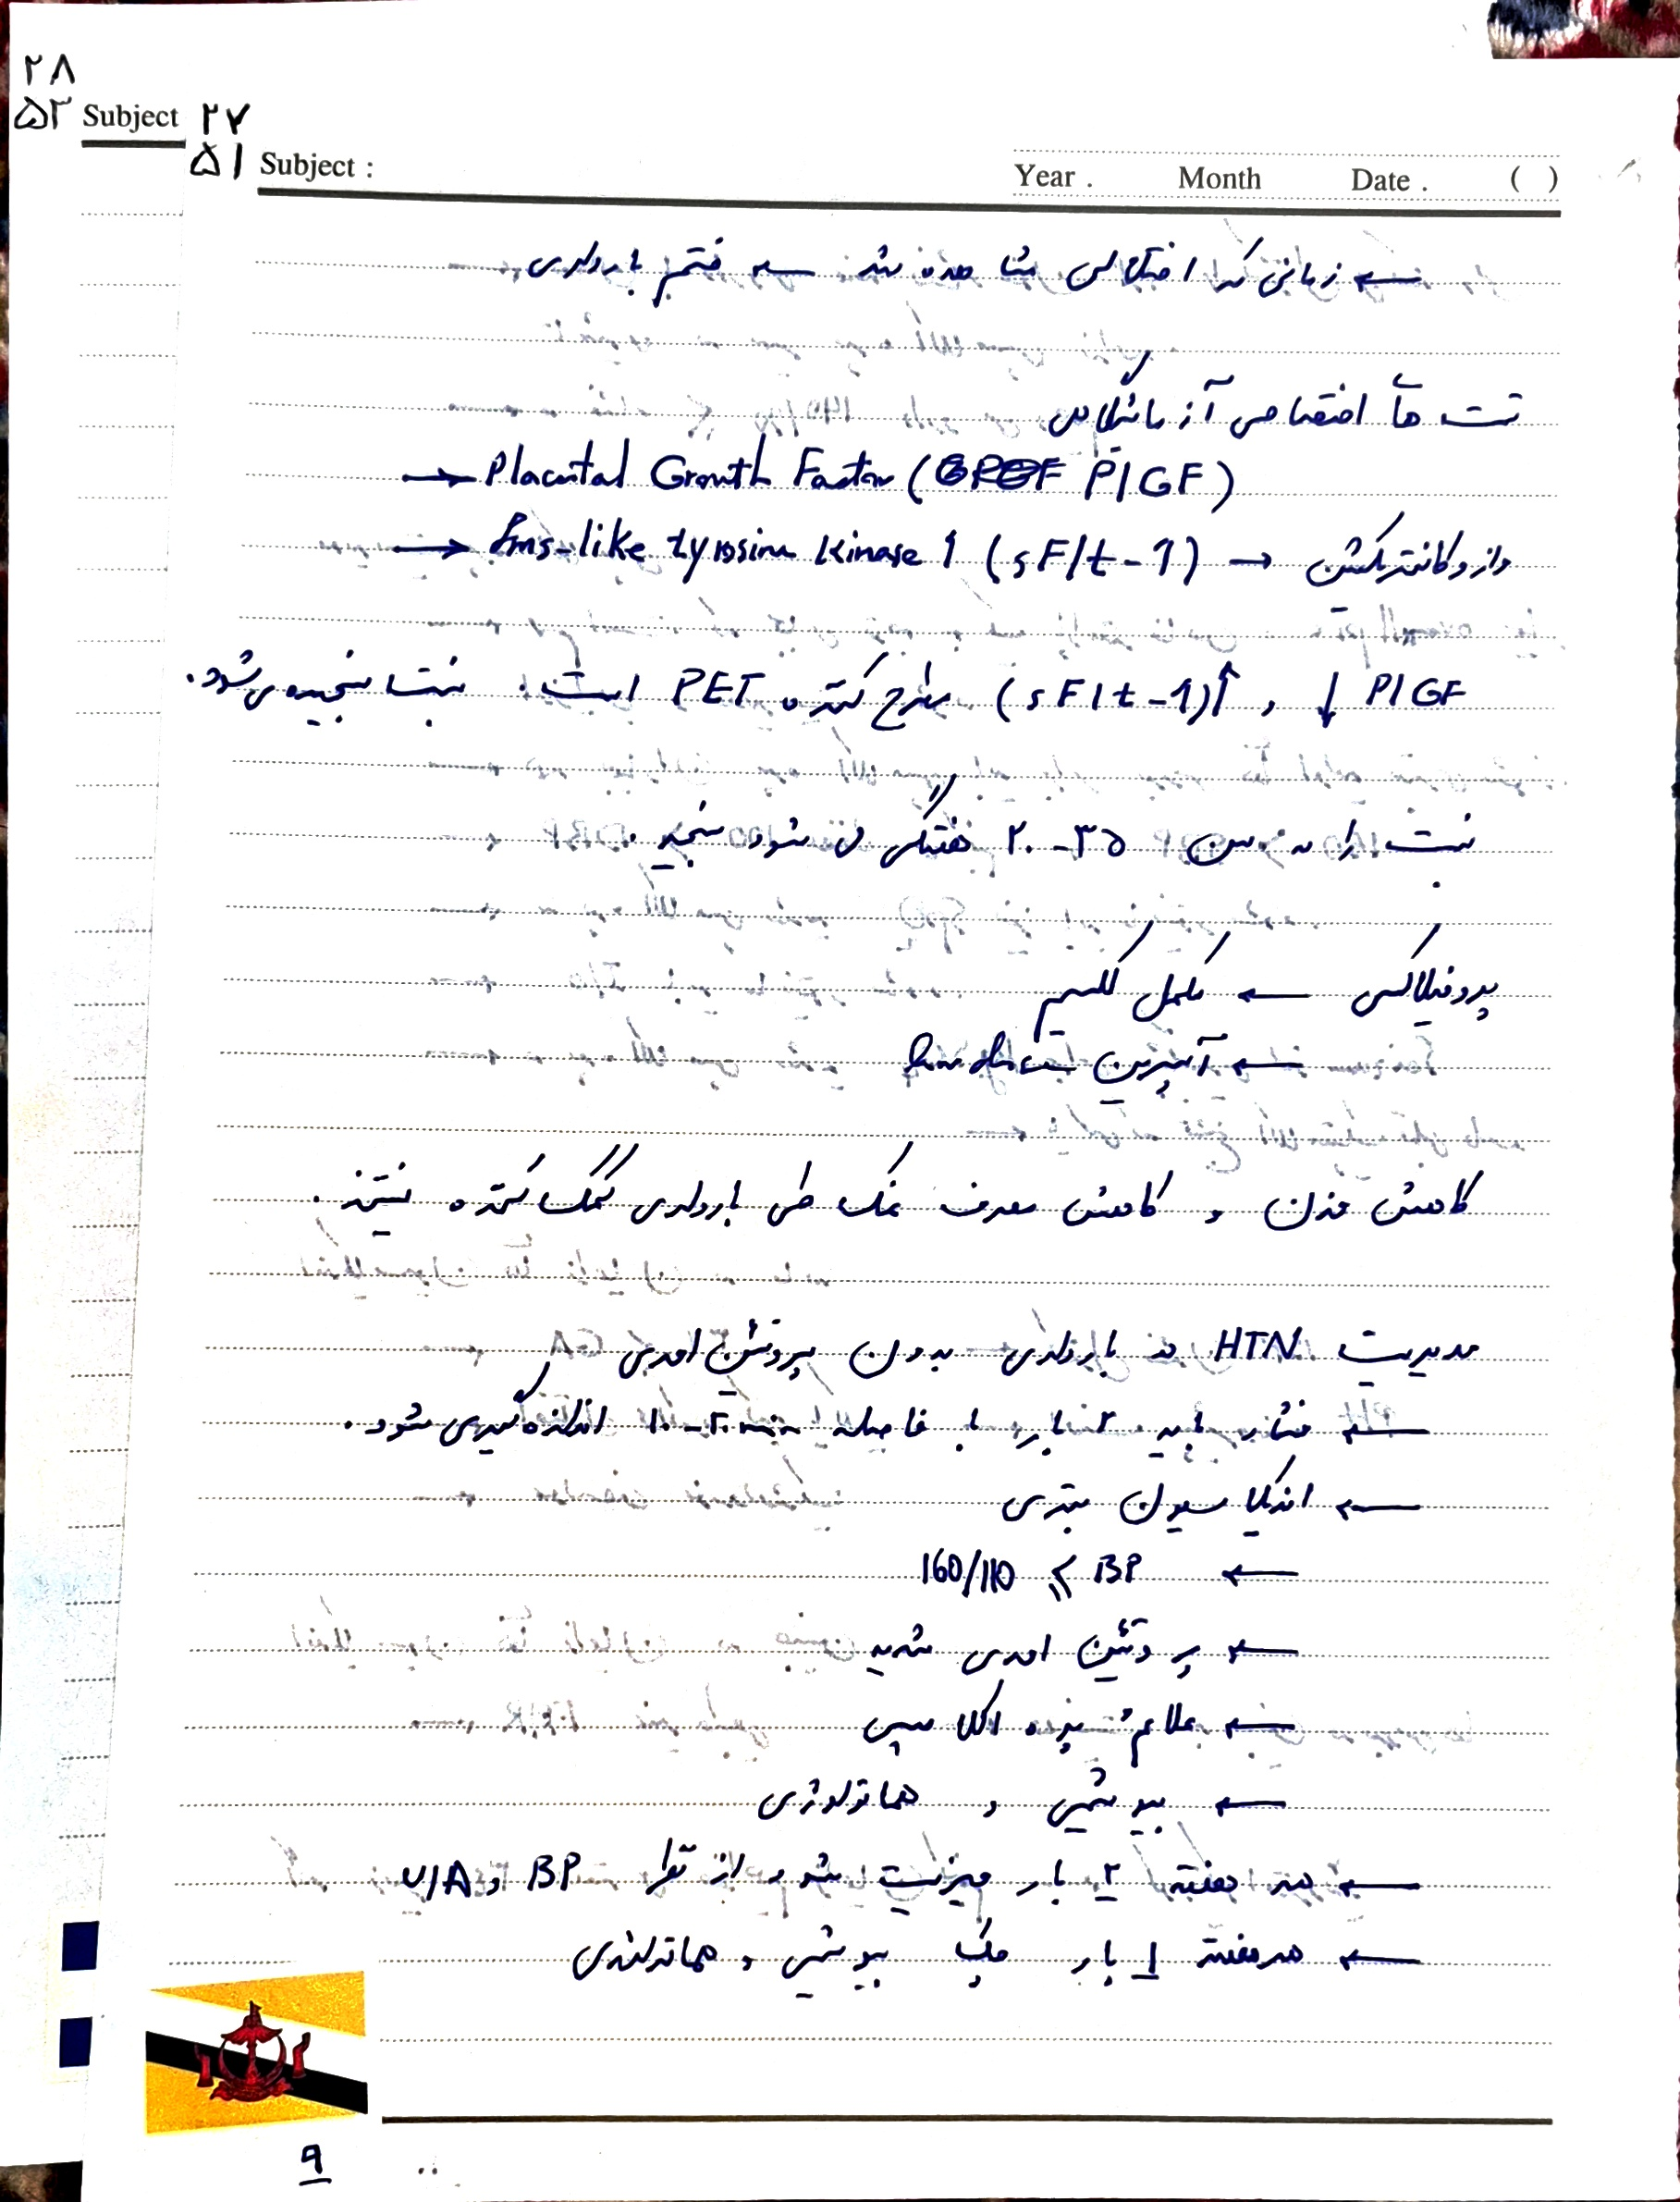
\includegraphics[width=\textwidth,height=0.86\textheight,keepaspectratio]{images/pic09.jpg}
\end{center}
% pic10.jpg = 20261013_024728978.jpg; Drive ID: 17RRZPOYUTwH9FblvbOxEwkAejjSjU3It
\clearpage
\begin{center}
\textbf{تصویر 10}\par
\lr{\detokenize{20261013_024728978.jpg}}\par
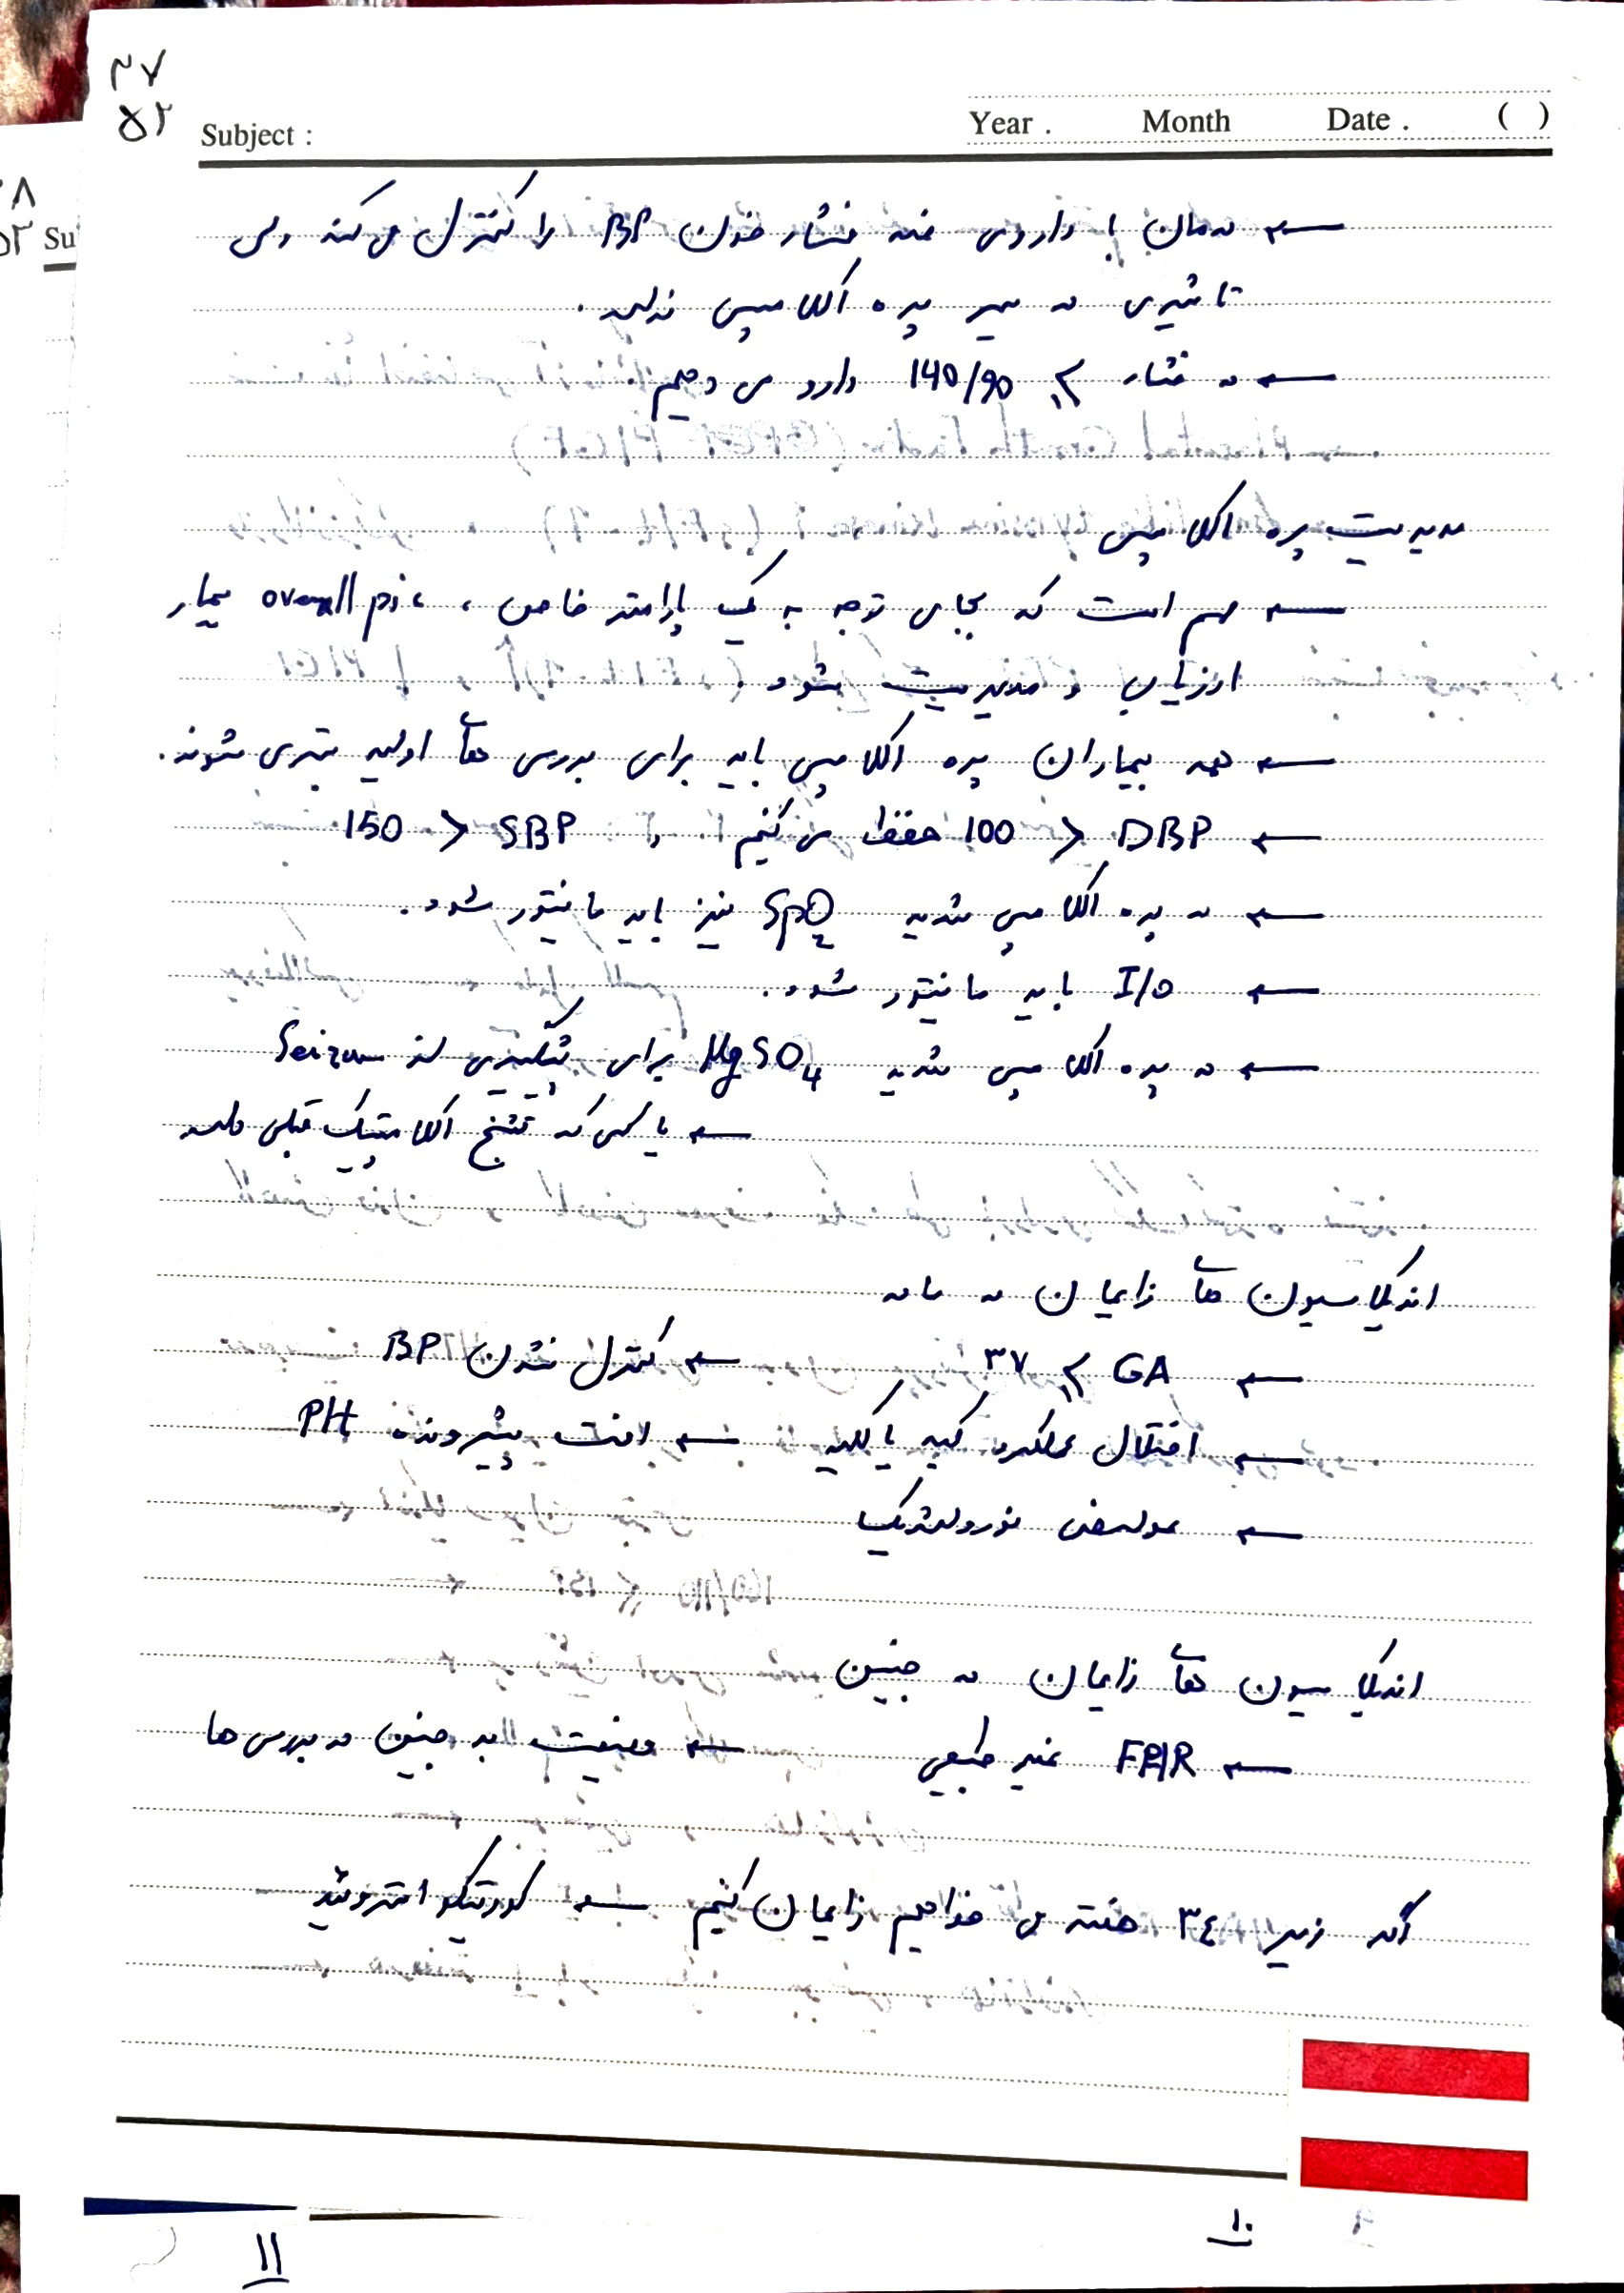
\includegraphics[width=\textwidth,height=0.86\textheight,keepaspectratio]{images/pic10.jpg}
\end{center}
% pic11.jpg = 20261013_024734607.jpg; Drive ID: 1A_FT945444WBds8Qv2rzoxzc6HKC2ls6
\clearpage
\begin{center}
\textbf{تصویر 11}\par
\lr{\detokenize{20261013_024734607.jpg}}\par
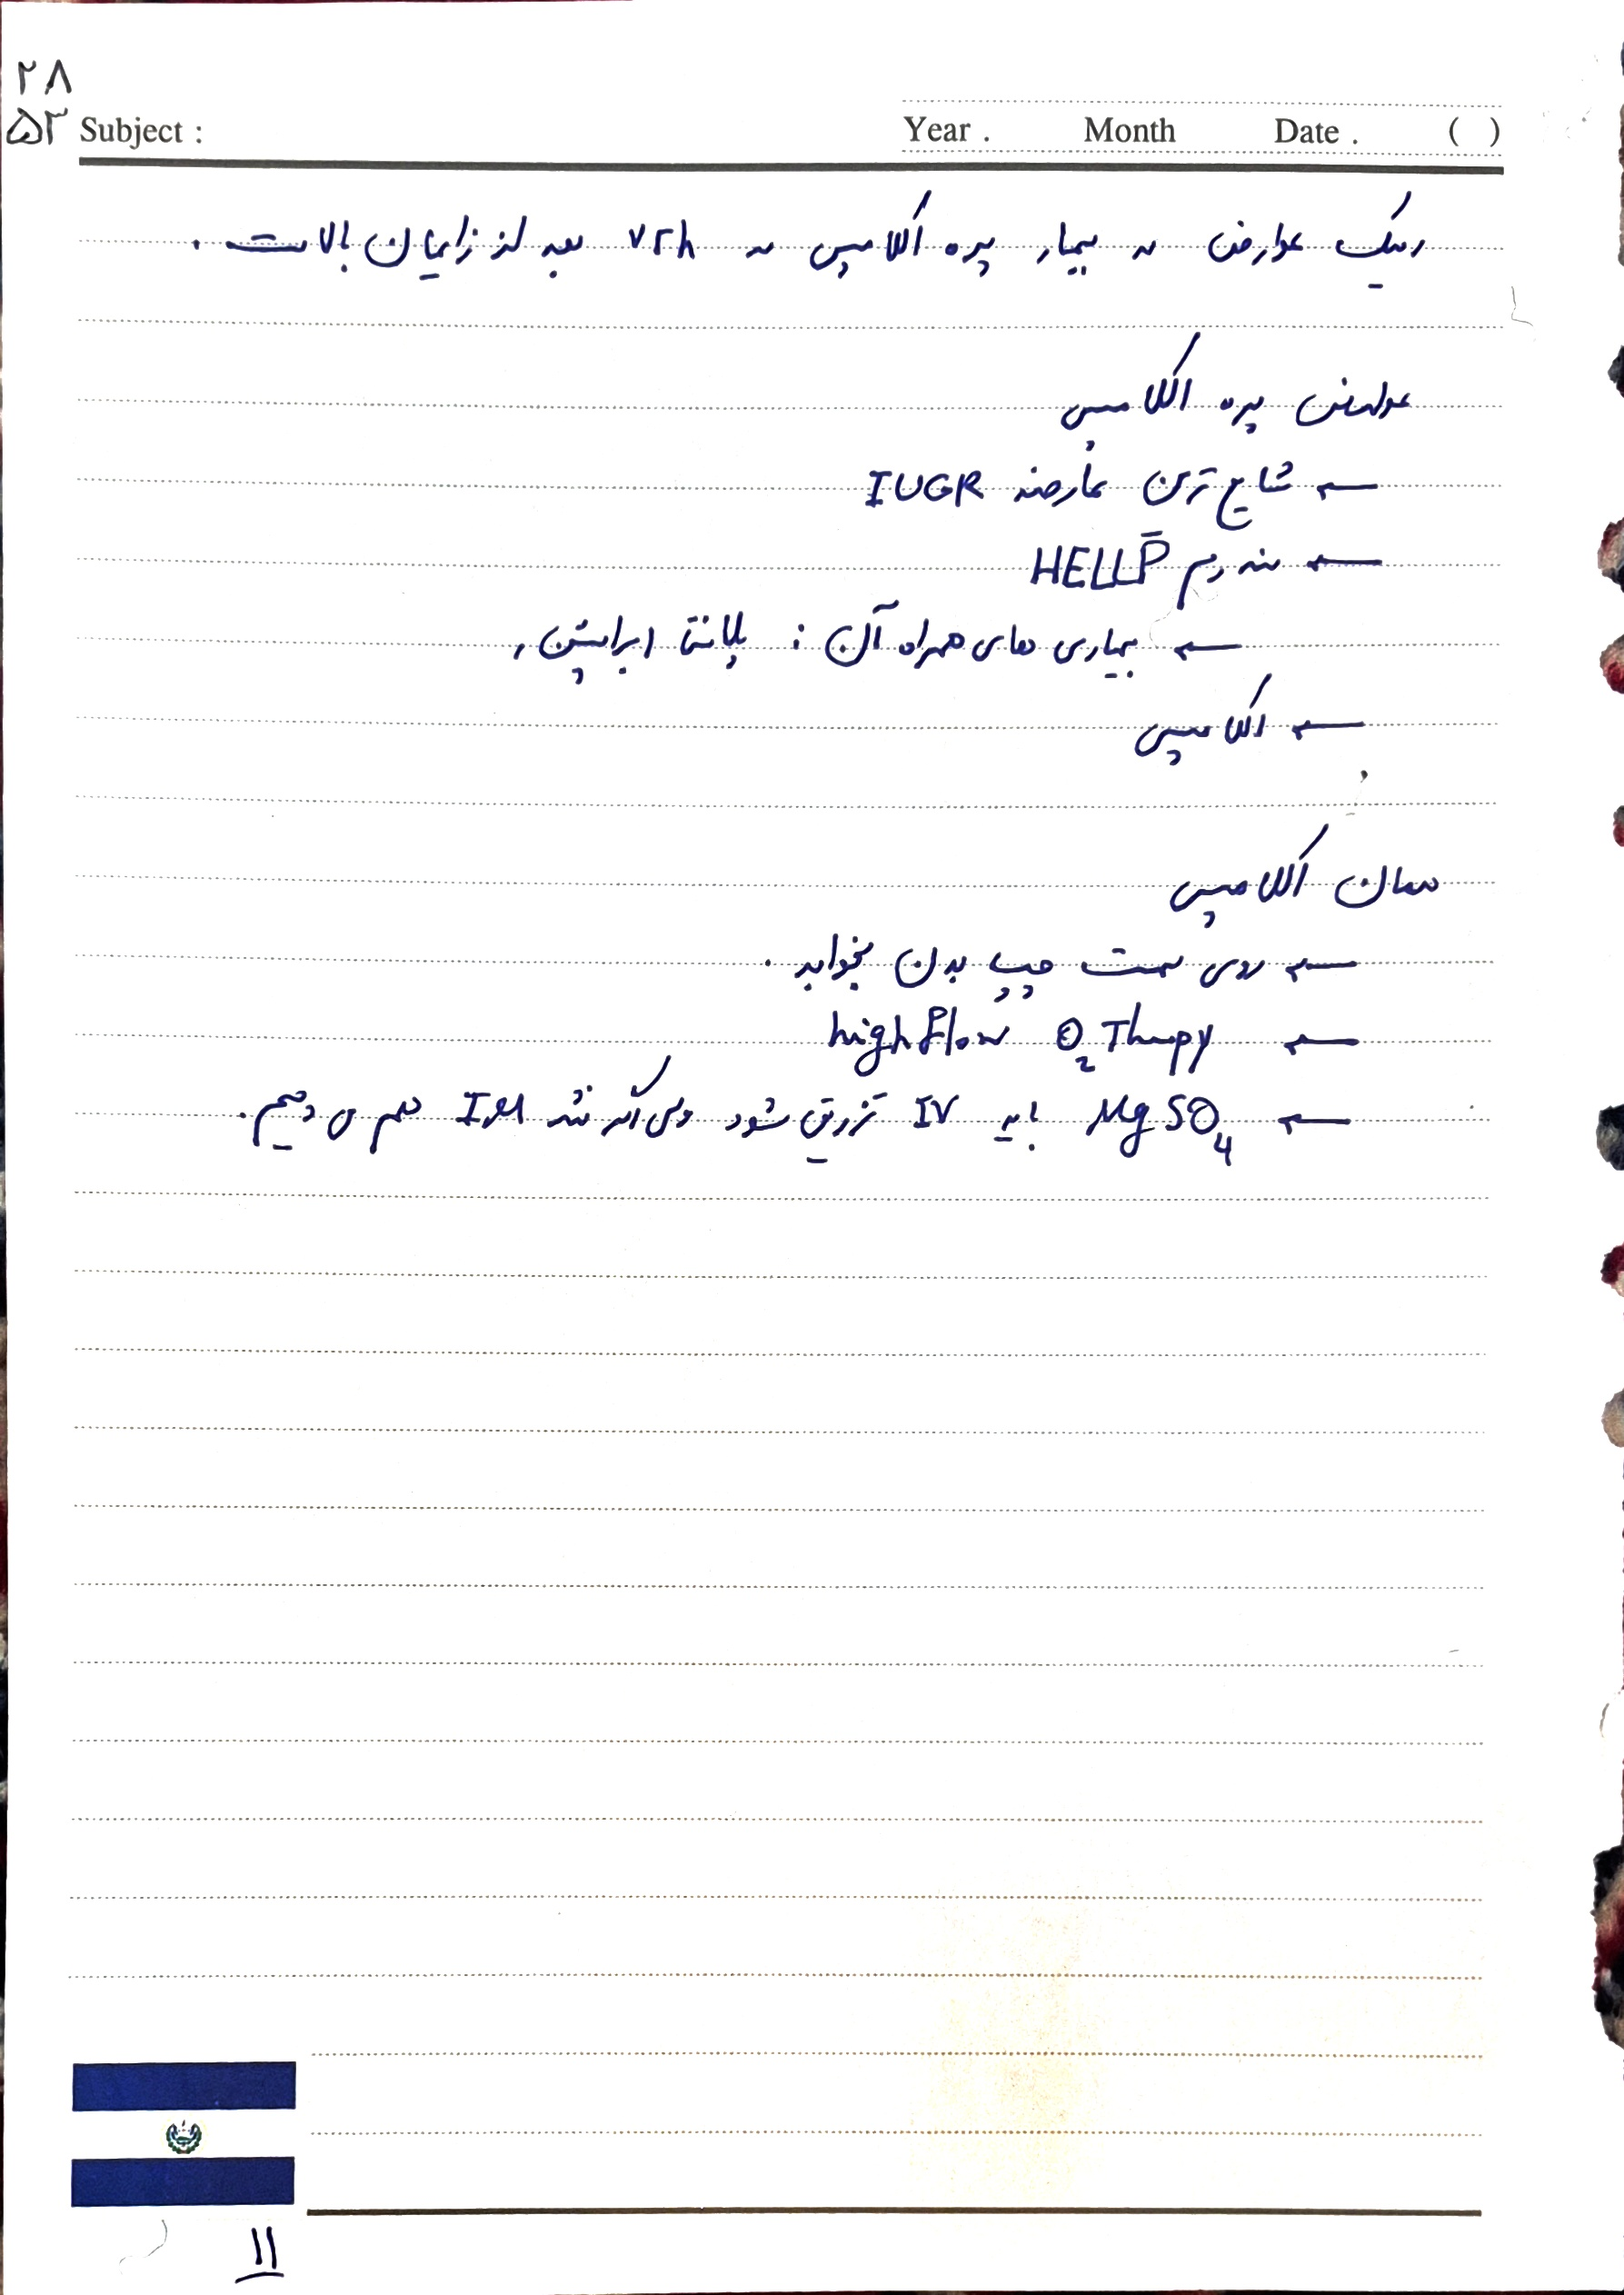
\includegraphics[width=\textwidth,height=0.86\textheight,keepaspectratio]{images/pic11.jpg}
\end{center}
\HTNfinish
